% Options for packages loaded elsewhere
% Options for packages loaded elsewhere
\PassOptionsToPackage{unicode}{hyperref}
\PassOptionsToPackage{hyphens}{url}
\PassOptionsToPackage{dvipsnames,svgnames,x11names}{xcolor}
%
\documentclass[
  letterpaper,
  DIV=11,
  numbers=noendperiod]{scrartcl}
\usepackage{xcolor}
\usepackage[top=15mm, bottom=25mm, left=10mm, right=10mm]{geometry}
\usepackage{amsmath,amssymb}
\setcounter{secnumdepth}{5}
\usepackage{iftex}
\ifPDFTeX
  \usepackage[T1]{fontenc}
  \usepackage[utf8]{inputenc}
  \usepackage{textcomp} % provide euro and other symbols
\else % if luatex or xetex
  \usepackage{unicode-math} % this also loads fontspec
  \defaultfontfeatures{Scale=MatchLowercase}
  \defaultfontfeatures[\rmfamily]{Ligatures=TeX,Scale=1}
\fi
\usepackage{lmodern}
\ifPDFTeX\else
  % xetex/luatex font selection
\fi
% Use upquote if available, for straight quotes in verbatim environments
\IfFileExists{upquote.sty}{\usepackage{upquote}}{}
\IfFileExists{microtype.sty}{% use microtype if available
  \usepackage[]{microtype}
  \UseMicrotypeSet[protrusion]{basicmath} % disable protrusion for tt fonts
}{}
\makeatletter
\@ifundefined{KOMAClassName}{% if non-KOMA class
  \IfFileExists{parskip.sty}{%
    \usepackage{parskip}
  }{% else
    \setlength{\parindent}{0pt}
    \setlength{\parskip}{6pt plus 2pt minus 1pt}}
}{% if KOMA class
  \KOMAoptions{parskip=half}}
\makeatother
% Make \paragraph and \subparagraph free-standing
\makeatletter
\ifx\paragraph\undefined\else
  \let\oldparagraph\paragraph
  \renewcommand{\paragraph}{
    \@ifstar
      \xxxParagraphStar
      \xxxParagraphNoStar
  }
  \newcommand{\xxxParagraphStar}[1]{\oldparagraph*{#1}\mbox{}}
  \newcommand{\xxxParagraphNoStar}[1]{\oldparagraph{#1}\mbox{}}
\fi
\ifx\subparagraph\undefined\else
  \let\oldsubparagraph\subparagraph
  \renewcommand{\subparagraph}{
    \@ifstar
      \xxxSubParagraphStar
      \xxxSubParagraphNoStar
  }
  \newcommand{\xxxSubParagraphStar}[1]{\oldsubparagraph*{#1}\mbox{}}
  \newcommand{\xxxSubParagraphNoStar}[1]{\oldsubparagraph{#1}\mbox{}}
\fi
\makeatother

\usepackage{color}
\usepackage{fancyvrb}
\newcommand{\VerbBar}{|}
\newcommand{\VERB}{\Verb[commandchars=\\\{\}]}
\DefineVerbatimEnvironment{Highlighting}{Verbatim}{commandchars=\\\{\}}
% Add ',fontsize=\small' for more characters per line
\usepackage{framed}
\definecolor{shadecolor}{RGB}{241,243,245}
\newenvironment{Shaded}{\begin{snugshade}}{\end{snugshade}}
\newcommand{\AlertTok}[1]{\textcolor[rgb]{0.68,0.00,0.00}{#1}}
\newcommand{\AnnotationTok}[1]{\textcolor[rgb]{0.37,0.37,0.37}{#1}}
\newcommand{\AttributeTok}[1]{\textcolor[rgb]{0.40,0.45,0.13}{#1}}
\newcommand{\BaseNTok}[1]{\textcolor[rgb]{0.68,0.00,0.00}{#1}}
\newcommand{\BuiltInTok}[1]{\textcolor[rgb]{0.00,0.23,0.31}{#1}}
\newcommand{\CharTok}[1]{\textcolor[rgb]{0.13,0.47,0.30}{#1}}
\newcommand{\CommentTok}[1]{\textcolor[rgb]{0.37,0.37,0.37}{#1}}
\newcommand{\CommentVarTok}[1]{\textcolor[rgb]{0.37,0.37,0.37}{\textit{#1}}}
\newcommand{\ConstantTok}[1]{\textcolor[rgb]{0.56,0.35,0.01}{#1}}
\newcommand{\ControlFlowTok}[1]{\textcolor[rgb]{0.00,0.23,0.31}{\textbf{#1}}}
\newcommand{\DataTypeTok}[1]{\textcolor[rgb]{0.68,0.00,0.00}{#1}}
\newcommand{\DecValTok}[1]{\textcolor[rgb]{0.68,0.00,0.00}{#1}}
\newcommand{\DocumentationTok}[1]{\textcolor[rgb]{0.37,0.37,0.37}{\textit{#1}}}
\newcommand{\ErrorTok}[1]{\textcolor[rgb]{0.68,0.00,0.00}{#1}}
\newcommand{\ExtensionTok}[1]{\textcolor[rgb]{0.00,0.23,0.31}{#1}}
\newcommand{\FloatTok}[1]{\textcolor[rgb]{0.68,0.00,0.00}{#1}}
\newcommand{\FunctionTok}[1]{\textcolor[rgb]{0.28,0.35,0.67}{#1}}
\newcommand{\ImportTok}[1]{\textcolor[rgb]{0.00,0.46,0.62}{#1}}
\newcommand{\InformationTok}[1]{\textcolor[rgb]{0.37,0.37,0.37}{#1}}
\newcommand{\KeywordTok}[1]{\textcolor[rgb]{0.00,0.23,0.31}{\textbf{#1}}}
\newcommand{\NormalTok}[1]{\textcolor[rgb]{0.00,0.23,0.31}{#1}}
\newcommand{\OperatorTok}[1]{\textcolor[rgb]{0.37,0.37,0.37}{#1}}
\newcommand{\OtherTok}[1]{\textcolor[rgb]{0.00,0.23,0.31}{#1}}
\newcommand{\PreprocessorTok}[1]{\textcolor[rgb]{0.68,0.00,0.00}{#1}}
\newcommand{\RegionMarkerTok}[1]{\textcolor[rgb]{0.00,0.23,0.31}{#1}}
\newcommand{\SpecialCharTok}[1]{\textcolor[rgb]{0.37,0.37,0.37}{#1}}
\newcommand{\SpecialStringTok}[1]{\textcolor[rgb]{0.13,0.47,0.30}{#1}}
\newcommand{\StringTok}[1]{\textcolor[rgb]{0.13,0.47,0.30}{#1}}
\newcommand{\VariableTok}[1]{\textcolor[rgb]{0.07,0.07,0.07}{#1}}
\newcommand{\VerbatimStringTok}[1]{\textcolor[rgb]{0.13,0.47,0.30}{#1}}
\newcommand{\WarningTok}[1]{\textcolor[rgb]{0.37,0.37,0.37}{\textit{#1}}}

\usepackage{longtable,booktabs,array}
\usepackage{calc} % for calculating minipage widths
% Correct order of tables after \paragraph or \subparagraph
\usepackage{etoolbox}
\makeatletter
\patchcmd\longtable{\par}{\if@noskipsec\mbox{}\fi\par}{}{}
\makeatother
% Allow footnotes in longtable head/foot
\IfFileExists{footnotehyper.sty}{\usepackage{footnotehyper}}{\usepackage{footnote}}
\makesavenoteenv{longtable}
\usepackage{graphicx}
\makeatletter
\newsavebox\pandoc@box
\newcommand*\pandocbounded[1]{% scales image to fit in text height/width
  \sbox\pandoc@box{#1}%
  \Gscale@div\@tempa{\textheight}{\dimexpr\ht\pandoc@box+\dp\pandoc@box\relax}%
  \Gscale@div\@tempb{\linewidth}{\wd\pandoc@box}%
  \ifdim\@tempb\p@<\@tempa\p@\let\@tempa\@tempb\fi% select the smaller of both
  \ifdim\@tempa\p@<\p@\scalebox{\@tempa}{\usebox\pandoc@box}%
  \else\usebox{\pandoc@box}%
  \fi%
}
% Set default figure placement to htbp
\def\fps@figure{htbp}
\makeatother


% definitions for citeproc citations
\NewDocumentCommand\citeproctext{}{}
\NewDocumentCommand\citeproc{mm}{%
  \begingroup\def\citeproctext{#2}\cite{#1}\endgroup}
\makeatletter
 % allow citations to break across lines
 \let\@cite@ofmt\@firstofone
 % avoid brackets around text for \cite:
 \def\@biblabel#1{}
 \def\@cite#1#2{{#1\if@tempswa , #2\fi}}
\makeatother
\newlength{\cslhangindent}
\setlength{\cslhangindent}{1.5em}
\newlength{\csllabelwidth}
\setlength{\csllabelwidth}{3em}
\newenvironment{CSLReferences}[2] % #1 hanging-indent, #2 entry-spacing
 {\begin{list}{}{%
  \setlength{\itemindent}{0pt}
  \setlength{\leftmargin}{0pt}
  \setlength{\parsep}{0pt}
  % turn on hanging indent if param 1 is 1
  \ifodd #1
   \setlength{\leftmargin}{\cslhangindent}
   \setlength{\itemindent}{-1\cslhangindent}
  \fi
  % set entry spacing
  \setlength{\itemsep}{#2\baselineskip}}}
 {\end{list}}
\usepackage{calc}
\newcommand{\CSLBlock}[1]{\hfill\break\parbox[t]{\linewidth}{\strut\ignorespaces#1\strut}}
\newcommand{\CSLLeftMargin}[1]{\parbox[t]{\csllabelwidth}{\strut#1\strut}}
\newcommand{\CSLRightInline}[1]{\parbox[t]{\linewidth - \csllabelwidth}{\strut#1\strut}}
\newcommand{\CSLIndent}[1]{\hspace{\cslhangindent}#1}



\setlength{\emergencystretch}{3em} % prevent overfull lines

\providecommand{\tightlist}{%
  \setlength{\itemsep}{0pt}\setlength{\parskip}{0pt}}



 


\usepackage{fvextra}
\DefineVerbatimEnvironment{Highlighting}{Verbatim}{breaklines,commandchars=\\\{\}}
\DefineVerbatimEnvironment{OutputCode}{Verbatim}{breaklines,commandchars=\\\{\}}
\KOMAoption{captions}{tableheading}
\makeatletter
\@ifpackageloaded{caption}{}{\usepackage{caption}}
\AtBeginDocument{%
\ifdefined\contentsname
  \renewcommand*\contentsname{Table of contents}
\else
  \newcommand\contentsname{Table of contents}
\fi
\ifdefined\listfigurename
  \renewcommand*\listfigurename{List of Figures}
\else
  \newcommand\listfigurename{List of Figures}
\fi
\ifdefined\listtablename
  \renewcommand*\listtablename{List of Tables}
\else
  \newcommand\listtablename{List of Tables}
\fi
\ifdefined\figurename
  \renewcommand*\figurename{Fig}
\else
  \newcommand\figurename{Fig}
\fi
\ifdefined\tablename
  \renewcommand*\tablename{Tbl}
\else
  \newcommand\tablename{Tbl}
\fi
}
\@ifpackageloaded{float}{}{\usepackage{float}}
\floatstyle{ruled}
\@ifundefined{c@chapter}{\newfloat{codelisting}{h}{lop}}{\newfloat{codelisting}{h}{lop}[chapter]}
\floatname{codelisting}{Listing}
\newcommand*\listoflistings{\listof{codelisting}{List of Listings}}
\makeatother
\makeatletter
\makeatother
\makeatletter
\@ifpackageloaded{caption}{}{\usepackage{caption}}
\@ifpackageloaded{subcaption}{}{\usepackage{subcaption}}
\makeatother
\usepackage{bookmark}
\IfFileExists{xurl.sty}{\usepackage{xurl}}{} % add URL line breaks if available
\urlstyle{same}
\hypersetup{
  pdftitle={AI-powered Qualitative Interviews and Focus Groups},
  pdfauthor={Torben Fischer},
  colorlinks=true,
  linkcolor={blue},
  filecolor={Maroon},
  citecolor={Blue},
  urlcolor={Blue},
  pdfcreator={LaTeX via pandoc}}


\title{AI-powered Qualitative Interviews and Focus
Groups\thanks{s72tfisc@uni-bonn.de, University of Bonn and Bonn Graduate
School of Economics (BGSE)}}
\usepackage{etoolbox}
\makeatletter
\providecommand{\subtitle}[1]{% add subtitle to \maketitle
  \apptocmd{\@title}{\par {\large #1 \par}}{}{}
}
\makeatother
\subtitle{prepared for the course `Data Science, Machine Learning, and
AI' held by Prof.~Thiemo Fetzer}
\author{Torben Fischer}
\date{2025-08-22}
\begin{document}
\maketitle
\begin{abstract}
This repository builds on previous work by Chopra and Haaland
(\citeproc{ref-chopra_haaland_2024}{2024}) and Geiecke and Jaravel
(\citeproc{ref-geiecke_jaravel_2025}{2025}) who introduced the new
methodology to conduct qualitative interviews by delegating the role of
the moderator to a well-prompted AI moderator. This deliverable extends
their work in two ways. Firstly, additional code allows to run the
qualitative AI-interviews using local, open-source AI models, e.g.,
gemma3, provided by Ollama, now. Secondly, as the main contribution of
this deliverable, the codebase creates a scalebale and cost-efficient
AI-moderated focus group discussion between several AI agents simulating
participants and optionally one human participant. A simple qualitative
analysis - using AI for topic modeling - shows that transcripts of AI
and human focus groups cover similar topics and themes. Links to try out
the AI-led qualitative interviews and AI-powered focus group (with or
without yourself as the human participant) are shared in
Section~\ref{sec-links}.
\end{abstract}

\renewcommand*\contentsname{Table of contents}
{
\hypersetup{linkcolor=}
\setcounter{tocdepth}{3}
\tableofcontents
}

\section{Motivation \& Introduction}\label{sec-introduction_motivation}

Qualitative methods are experiencing a resurgence in the social
sciences. While computational advances have long supported the analysis
of qualitative data, only recent breakthroughs in Artificial
Intelligence (AI) have made qualitative research scalable. In
experimental economics, for example, applications were traditionally
confined to single open-ended survey questions. As Haaland et al.
(\citeproc{ref-haaland_roth_stantcheva_wohlfahrt_forthcoming}{forthcoming})
note, such methods are valuable for uncovering pieces of narratives,
mechanisms, and reasoning, but remain limited to \emph{top-of-mind}
responses. Thus, there is a need for the application of more elaborate
methods. A natural extension of single open-ended questions is the
method of semi-structured \textbf{qualitative interviews}, usually
guided by a topic outline. These interviews have generated important
insights, such as explaining why low-income families often remain in
low-opportunity neighborhoods
(\citeproc{ref-bergman_chetty_deluca_hendren_katz_palmer_2024}{Bergman
et al. 2024}), but their widespread use is constrained by high costs and
incompatibility with experimental or survey designs.

To address these barriers, Chopra and Haaland
(\citeproc{ref-chopra_haaland_2024}{2024}) and Geiecke and Jaravel
(\citeproc{ref-geiecke_jaravel_2025}{2025}) pioneered AI-led qualitative
interviews, in which a well-prompted AI agent acts as the interviewer.
This design reduces both, interviewer and interviewee social
desirability bias
(\citeproc{ref-bursztyn_haaland_roever_roth_2025}{Bursztyn et al. 2025})
and, strikingly, is even weakly preferred by participants over human-led
interviews. The papers showcase that AI-led qualitative interviews are
able to reveal unknown mental models explaining why people are reluctant
to invest and create a deeper understanding of voting decisions.

This deliverable builds directly on the code of Geiecke and Jaravel
(\citeproc{ref-geiecke_jaravel_2025}{2025}) and extends it to a
\textbf{focus group} format.

Focus groups are a cornerstone of qualitative research in health and
social care (\citeproc{ref-rabiee_2004}{Rabiee 2004}), marketing, and
policy evaluation (\citeproc{ref-kahan_2001}{Kahan 2001}). They
typically bring together 6--12 participants for 60--90 minutes of
semi-structured discussion, moderated through a guide that balances
structure with open dialogue. The format is particularly effective at
eliciting collective perspectives, surfacing social dynamics, and
probing motivations and decision-making processes
(\citeproc{ref-billups_2021}{Billups 2021}).

The AI-led focus group created here reproduces this format with an AI
moderator and AI-simulated participants, optionally combined with a
human participant. This approach offers four key advantages:

\textbf{1. Scalability and efficiency:} Sessions can be conducted
quickly and at low cost. There are (almost) no people that have to be
paid. A pure AI focus group that lasts 60 minutes costs about between
\$1 and \$2.

\textbf{2. Consistency and adaptability:} AI moderators do not suffer
from behavioral biases and remain tireless, no matter how long the
discussion is already ongoing.

\textbf{3. Diversity of perspectives:} AI participants, designed to
reflect different stakeholder positions or trained on broad datasets,
likely introduce novel or underexplored viewpoints.

\textbf{4. Flexible group composition:} Homogeneous or heterogeneous
groups can be assembled instantly, bypassing recruitment challenges.
Also the moderator has not to be trained on the topic first.

By combining the depth of traditional focus groups with the scalability
of AI, this method opens new possibilities for exploring ``what-if''
scenarios, testing reactions to emerging issues, and generating richer,
more diverse qualitative insights. In particular, we show that the here
constructed AI focus group performs similarly to human focus groups
outputwise.

The deliverable is structured as follows. To give you and idea what the
deliverable/repository does, we offer you to run both AI-led qualitative
interviews, as well as both versions of the AI-powered focus group in
Section~\ref{sec-links}. Section~\ref{sec-replication} provides an
overview and instructions for replicating and setting up the AI-led
qualitative interviews developed by Chopra and Haaland
(\citeproc{ref-chopra_haaland_2024}{2024}) and Geiecke and Jaravel
(\citeproc{ref-geiecke_jaravel_2025}{2025}), both locally and globally.
Section~\ref{sec-focusgroup} then introduces the main contribution of
this deliverable: code for configuring an AI-moderated focus group
discussion with additional AI agents simulating participants, alongside
the option of including a human participant. This section also details
the key coding and prompting choices, while addressing limitations and
outlining potential extensions. Section~\ref{sec-evaluation} assesses
the quality of the fully AI-based focus group by comparing the topics
and themes it generates with those emerging from human focus group
interactions reported in Morton et al.
(\citeproc{ref-morton_fitzsimons_sivaramakrishan_jepson_niven_2024}{2024}).
Finally, Section~\ref{sec-discussion} concludes by summarizing the
strengths and weaknesses of the AI focus group format presented here.

\section{Links}\label{sec-links}

This section allows you to explore both AI-led qualitative interviews
and AI-powered focus groups, with or without a human participant.

\begin{enumerate}
\def\labelenumi{\arabic{enumi}.}
\tightlist
\item
  AI-Led Qualitative Interviews
\end{enumerate}

We use the default interviews implemented in the respective
repositories:

\begin{itemize}
\item
  Chopra and Haaland (\citeproc{ref-chopra_haaland_2024}{2024}): The
  interview focuses on the participation puzzle --- why do people not
  invest in stocks or mutual funds? The topic guide consists of almost
  20 questions.
\item
  Geiecke and Jaravel (\citeproc{ref-geiecke_jaravel_2025}{2025}): The
  interview explores your educational journey and its determinants. The
  topic guide consists of approximately 35 questions.
\end{itemize}

\begin{enumerate}
\def\labelenumi{\arabic{enumi}.}
\setcounter{enumi}{1}
\tightlist
\item
  AI-Powered Focus Group
\end{enumerate}

For the focus group, an exemplary scenario was coded around the topic
\emph{Reducing sedentary behavior while working from home: How can we
promote healthier and more active remote work routines?}

\begin{itemize}
\item
  This setup was inspired by research from Morton et al.
  (\citeproc{ref-morton_fitzsimons_sivaramakrishan_jepson_niven_2024}{2024}).
\item
  The AI focus group can be run with or without a human participant.
\item
  The session typically without a human lasts 5--10 minutes, but if
  translated into spoken words, it roughly equates to 60 minutes of
  discussion.
\end{itemize}

You can try the \emph{AI-led qualitative interview} designed by Chopra
and Haaland (\citeproc{ref-chopra_haaland_2024}{2024})
\href{https://tdbdo90q9g.execute-api.eu-north-1.amazonaws.com/default/qualtricsRedirectHandler}{here}.

You can try the \emph{AI-led qualitative interview} designed by Geiecke
and Jaravel (\citeproc{ref-geiecke_jaravel_2025}{2025})
\href{https://ai-led-interview.streamlit.app/}{here}.

You can try the \emph{AI-powered focus group} \textbf{without} a
\emph{human participant} \href{https://focusgroup.streamlit.app/}{here}.

You can try the \emph{AI-powered focus group} \textbf{with} a
\emph{human participant}
\href{https://focusgroup-human.streamlit.app/}{here}.

These examples are running using my API keys. If you encounter any
issues, such as the examples not working because the API key has run out
of credits, please contact me at \texttt{s72tfisc@uni-bonn.de}. However,
there should be enough credits for at least 30 trys so that this is
unlikely to occur.

\section{Replication}\label{sec-replication}

This section replicates the AI-led qualitative interview designed by
Chopra and Haaland (\citeproc{ref-chopra_haaland_2024}{2024}) and
Geiecke and Jaravel (\citeproc{ref-geiecke_jaravel_2025}{2025}).

\subsection{Comparison of AI-led Interview
Implementations}\label{comparison-of-ai-led-interview-implementations}

Both Chopra and Haaland (\citeproc{ref-chopra_haaland_2024}{2024}) and
Geiecke and Jaravel (\citeproc{ref-geiecke_jaravel_2025}{2025}) follow a
similar conceptual approach, using \textbf{OpenAI API Keys} combined
with a \texttt{chat-gpt-4o} model to conduct AI-led qualitative
interviews. Both codebases perform equally fine from my perspective.
However, there are minor differences in their architecture, performance,
and implementation style.

\begin{enumerate}
\def\labelenumi{\arabic{enumi}.}
\tightlist
\item
  \textbf{Token Management and Multi-Agent Architecture}

  \begin{itemize}
  \tightlist
  \item
    \textbf{Chopra and Haaland
    (\citeproc{ref-chopra_haaland_2024}{2024})}: Being the first to
    develop AI-led interviews, they faced challenges with token limits
    in long conversations. To overcome this, they implemented a
    \textbf{multi-AI-agent architecture} that summarizes context and
    conversation flow across multiple agents.\\
  \item
    \textbf{Geiecke and Jaravel
    (\citeproc{ref-geiecke_jaravel_2025}{2025})}: This architecture is
    no longer necessary. They simplify the setup by using a single AI
    agent - in particular the \texttt{messages} input of the moderator
    prompt - benefiting from more efficient token usage.
  \end{itemize}
\item
  \textbf{Response Streaming}

  \begin{itemize}
  \tightlist
  \item
    \textbf{Geiecke and Jaravel
    (\citeproc{ref-geiecke_jaravel_2025}{2025})}: Implements
    \textbf{streaming of AI responses}, which allows participants to see
    answers as they are generated. This enhances interactivity and
    reduces waiting time.\\
  \item
    \textbf{Chopra and Haaland
    (\citeproc{ref-chopra_haaland_2024}{2024})}: Uses a more traditional
    response model, which may have slightly longer latency for each AI
    reply.
  \end{itemize}
\item
  \textbf{Application Framework}

  \begin{itemize}
  \tightlist
  \item
    \textbf{Chopra and Haaland
    (\citeproc{ref-chopra_haaland_2024}{2024})}: Built on a
    \textbf{Flask app}, providing a classic web server setup suitable
    for flexible backend integrations and deployment (e.g., on AWS
    Lambda). The app setup is based on JSON and HTML, making the design
    of the app more complex, but also easier to edit.
  \item
    \textbf{Geiecke and Jaravel
    (\citeproc{ref-geiecke_jaravel_2025}{2025})}: Uses a
    \textbf{Streamlit app}, offering faster setup for local or online
    deployment with an interactive interface out-of-the-box. This does
    not need any JSON or HTML input, and therefore is especially
    convenient for rapid prototyping and testing.
  \end{itemize}
\end{enumerate}

\subsection{\texorpdfstring{Chopra and Haaland
(\citeproc{ref-chopra_haaland_2024}{2024})}{Chopra and Haaland (2024)}}\label{sec-replication-chopra}

The codebase to replicate Chopra and Haaland
(\citeproc{ref-chopra_haaland_2024}{2024}) is stored in the folder
\texttt{Chopra\_Haaland\_2024} of this repository.\\
If you want to work with the original code, you can clone Felix Chopra's
\href{https://github.com/fchop/interviews}{repository}.\\
Since no relevant changes were made to the code, the following steps
should work in both cases.\\
You may also follow the instructions given in Chopra's repo --- most
parts are identical --- but here I provide additional information for
the global setup.

Once you have cloned one of the repositories, you can set up the AI-led
qualitative interview either \textbf{locally} or \textbf{globally
(online)} by following the steps below.

\textbf{Step 0: OpenAI API Keys}

This AI-led qualitative interview template requires OpenAI API keys.\\
Before you start, replace the placeholder credentials in
\texttt{app/app.py}. Otherwise, the interviewer will not respond.

If you don't have an API key yet, you can create one
\href{https://platform.openai.com/settings/organization/api-keys}{here}.

\textbf{Note:} If you have used OpenAI in Python before, you might need
to uninstall \texttt{openai} and install an older version, since newer
versions may not support the syntax used for API calls.

\textbf{Step 1: Local Environment}

For both local and global setups, first create a virtual environment and
install the required packages:

\begin{Shaded}
\begin{Highlighting}[]
\ExtensionTok{python} \AttributeTok{{-}m}\NormalTok{ venv interviews{-}env}
\BuiltInTok{cd}\NormalTok{ interviews{-}env}
\BuiltInTok{source}\NormalTok{ bin/activate}
\ExtensionTok{pip}\NormalTok{ install }\AttributeTok{{-}r}\NormalTok{ local\_requirements.txt}
\end{Highlighting}
\end{Shaded}

\subsubsection{Local Setup}\label{sec-replication-chopra-local}

\textbf{Step 2: Deploy App}

To host the app locally, you have to setup a development server:

\begin{Shaded}
\begin{Highlighting}[]
\ExtensionTok{python}\NormalTok{ app/app.py}
\end{Highlighting}
\end{Shaded}

The application is hosted at http://127.0.0.1:8000. By default, this
page only displays the message Running. To start an interview, you need
to extend the URL with two parameters:

\begin{enumerate}
\def\labelenumi{\arabic{enumi}.}
\item
  Interview key -- identifies which interview prompt template to use
  (e.g., the default is \texttt{STOCK\_MARKET}).
\item
  Session ID -- a unique string to distinguish your session.
\end{enumerate}

This is necessary because \texttt{app/app.py} can contain multiple
prompt templates for different qualitative interviews. For example,
navigating to:

\begin{Shaded}
\begin{Highlighting}[]
\NormalTok{http://127.0.0.1:8000/STOCK\_MARKET/TEST{-}SESSION{-}ID{-}123}
\end{Highlighting}
\end{Shaded}

will open a working interview session, where you can interact with the
AI interviewer in the role of the interviewee. You can stop the
development server at any time by pressing \texttt{Ctrl} + \texttt{C} in
the terminal. All interview transcripts are automatically saved in the
\texttt{app/data} folder.

\subsubsection{Global Setup}\label{sec-replication-chopra-global}

To host the app globally, you have two main options:

\begin{enumerate}
\def\labelenumi{\arabic{enumi}.}
\item
  Deploy the interview as a \textbf{Flask App} on your own server (see
  \href{https://github.com/fchop/interviews}{Felix Chopra's
  repository}).
\item
  Deploy the interview as an \textbf{AWS Lambda function} using a
  serverless architecture.
\end{enumerate}

This section explains how to deploy the application with \textbf{AWS
Lambda}, which avoids the need to manage your own server and scales
automatically.

(It might be useful to install
\href{https://docs.docker.com/engine/install/}{Docker} and open Docker
Desktop during the installation as the deployment works via a Docker
container.)

\textbf{Step 2: AWS Account \& Credentials}

If you do not already have an AWS account, create one here:
\href{https://signin.aws.amazon.com/signup?request_type=register}{AWS
Sign Up}.

\emph{IAM Users and Roles}

In AWS, it is considered best practice \emph{not to use your root
account credentials} for deployments. Instead, create an \emph{IAM User}
and assign it the necessary permissions, ideally through an \emph{IAM
Role}.\\
- \emph{IAM User} is a user identity for programmatic or console
access.\\
- \emph{IAM Role} is a set of permissions that can be assumed by users,
applications, or services.

By granting your IAM User the right IAM Role, you ensure the principle
of least privilege (only the permissions needed are given).

\emph{Access Keys}

To interact with AWS services programmatically, you need an \emph{Access
Key ID} and a \emph{Secret Access Key}:\\
- \emph{Access Key ID}: Like a username (public).\\
- \emph{Secret Access Key}: Like a password (private).

You can create and download these credentials from the \emph{IAM
Console} for your \emph{IAM User} (under \emph{Security Credentials}).\\
These keys are required to tunnel your application to AWS.

Replace the placeholders in the \texttt{app/lambda.py} file with your
access keys. This will allow your application to establish a secure
connection (``tunnel'') to AWS Lambda.

\textbf{Step 3: Install the AWS SAM CLI}

Since you will be deploying a \emph{serverless application}, you need
the \emph{AWS Serverless Application Model (SAM) CLI}. SAM provides
tooling to build, test, and deploy Lambda-based applications, along with
resources such as \emph{API Gateway} (for REST endpoints) and
\emph{DynamoDB} (for structured data storage).

Install SAM with:

\begin{Shaded}
\begin{Highlighting}[]
\ExtensionTok{pip}\NormalTok{ install aws{-}sam{-}cli}
\end{Highlighting}
\end{Shaded}

\textbf{Step 4: Create an AWS S3 Storage Bucket}

Because the server infrastructure is outsourced to AWS, you need a
reliable place to store the transcripts of your interviews.\\
For this, use a \emph{AWS S3 Storage Bucket}. The S3 bucket will hold
all interview session data and can later be accessed by your Lambda
function.

Note: You only need to create the S3 bucket once. After that, all
deployments can reuse it.

\emph{Option A: Using the provided setup script}

\begin{Shaded}
\begin{Highlighting}[]
\ExtensionTok{./aws\_setup.sh} \OperatorTok{\textless{}}\NormalTok{AWS\_ACCESS\_KEY\_ID}\OperatorTok{\textgreater{}} \OperatorTok{\textless{}}\NormalTok{AWS\_SECRET\_ACCESS\_KEY}\OperatorTok{\textgreater{}} \OperatorTok{\textless{}}\NormalTok{AWS\_REGION}\OperatorTok{\textgreater{}} \OperatorTok{\textless{}}\NormalTok{S3\_BUCKET}\OperatorTok{\textgreater{}}
\end{Highlighting}
\end{Shaded}

\emph{Option B: Using the AWS CLI directly}

\begin{Shaded}
\begin{Highlighting}[]
\ExtensionTok{aws}\NormalTok{ s3api create{-}bucket }\DataTypeTok{\textbackslash{}}
  \AttributeTok{{-}{-}bucket} \OperatorTok{\textless{}}\NormalTok{S3\_BUCKET}\OperatorTok{\textgreater{}} \DataTypeTok{\textbackslash{}}
  \AttributeTok{{-}{-}region} \OperatorTok{\textless{}}\NormalTok{AWS\_REGION}\OperatorTok{\textgreater{}} \DataTypeTok{\textbackslash{}}
  \AttributeTok{{-}{-}create{-}bucket{-}configuration}\NormalTok{ LocationConstraint=}\OperatorTok{\textless{}}\NormalTok{AWS\_REGION}\OperatorTok{\textgreater{}}
\end{Highlighting}
\end{Shaded}

Note: In addition to S3, the setup creates a DynamoDB table named
\texttt{interview-sessions} by default.

\textbf{Step 5: Deploy Lambda Function}

Now that you have your S3 bucket, you can deploy the interview
application as a Lambda function. Lambda allows you to run the app
without managing servers, and it integrates with API Gateway to provide
a public HTTP endpoint.

Run the deployment script:

\begin{Shaded}
\begin{Highlighting}[]
\ExtensionTok{./aws\_deploy.sh} \OperatorTok{\textless{}}\NormalTok{S3\_BUCKET}\OperatorTok{\textgreater{}}
\end{Highlighting}
\end{Shaded}

This will return your public endpoint URL:

\begin{Shaded}
\begin{Highlighting}[]
\ExtensionTok{{-}{-}{-}{-}{-}{-}{-}{-}{-}{-}{-}{-}{-}{-}{-}{-}{-}{-}{-}{-}{-}{-}{-}{-}{-}{-}{-}{-}{-}{-}{-}{-}{-}{-}{-}{-}{-}{-}{-}{-}{-}{-}{-}{-}{-}{-}{-}{-}{-}{-}{-}{-}{-}{-}{-}{-}{-}{-}{-}{-}{-}{-}{-}{-}{-}{-}{-}{-}{-}{-}{-}{-}{-}{-}{-}{-}{-}{-}}
\ExtensionTok{Outputs}
\ExtensionTok{{-}{-}{-}{-}{-}{-}{-}{-}{-}{-}{-}{-}{-}{-}{-}{-}{-}{-}{-}{-}{-}{-}{-}{-}{-}{-}{-}{-}{-}{-}{-}{-}{-}{-}{-}{-}{-}{-}{-}{-}{-}{-}{-}{-}{-}{-}{-}{-}{-}{-}{-}{-}{-}{-}{-}{-}{-}{-}{-}{-}{-}{-}{-}{-}{-}{-}{-}{-}{-}{-}{-}{-}{-}{-}{-}{-}{-}{-}}
\ExtensionTok{Key}\NormalTok{         InterviewApi}
\ExtensionTok{Description}\NormalTok{ API Gateway endpoint URL for function}
\ExtensionTok{Value}\NormalTok{       https://}\OperatorTok{\textless{}}\NormalTok{SOME\_AWS\_ID}\OperatorTok{\textgreater{}}\NormalTok{.execute{-}api.}\OperatorTok{\textless{}}\NormalTok{AWS\_REGION}\OperatorTok{\textgreater{}}\NormalTok{.amazonaws.com/Prod/}
\ExtensionTok{{-}{-}{-}{-}{-}{-}{-}{-}{-}{-}{-}{-}{-}{-}{-}{-}{-}{-}{-}{-}{-}{-}{-}{-}{-}{-}{-}{-}{-}{-}{-}{-}{-}{-}{-}{-}{-}{-}{-}{-}{-}{-}{-}{-}{-}{-}{-}{-}{-}{-}{-}{-}{-}{-}{-}{-}{-}{-}{-}{-}{-}{-}{-}{-}{-}{-}{-}{-}{-}{-}{-}{-}{-}{-}{-}{-}{-}{-}}
\end{Highlighting}
\end{Shaded}

You can now use the given API Gateway URL as the entry point to your
globally accessible interview application. For example:

\begin{verbatim}
https://<SOME_AWS_ID>.execute-api.<AWS_REGION>.amazonaws.com/Prod/STOCK_MARKET/TEST-SESSION-ID-123
\end{verbatim}

\textbf{Step 6: Qualtrics Integration}

An advantage of Chopra and Haaland
(\citeproc{ref-chopra_haaland_2024}{2024}) is that it is highly
compatible with survey platforms and can be easily integrated into
survey designs.\\
In particular, the AI-led interview can be embedded into
\href{https://login.qualtrics.com/login}{Qualtrics}, a widely used
platform for creating and publishing surveys.\\
In Qualtrics, \texttt{Text/Graphic} questions support editing via
\emph{JSON} and \emph{HTML} code. Note, however, that \emph{HTML
customizations are not available in the free version} of Qualtrics.

Chopra and Haaland (\citeproc{ref-chopra_haaland_2024}{2024}) provides
both JSON and HTML code that replicates the same chat interface used in
the local setup of the interview (see the folder \texttt{Qualtrics}).\\
Additionally, the setup allows you to choose between a text-only
interface or a voice-enabled interface for participants, depending on
your study requirements.

The connection between AWS and Qualtrics is established via the public
endpoint of your hosted application (see the \texttt{Value} field in the
Outputs of Step 5).\\
To integrate this endpoint into the survey, add an \emph{embedded
variable} \texttt{interview\_endpoint} in the Qualtrics survey flow.

\textbf{Step 7: Publishing Interview \& Redirection Handler (API
Gateway)}

From Qualtrics, the interview can be published, meaning that Qualtrics
generates a link that can be shared with participants.

However, to assign a \emph{unique link to each subject}, there are two
possible approaches:\\
1. \emph{Redirection handler} -- Create a handler that redirects each
participant to a unique session.\\
2. \emph{Embedded variables in the Qualtrics survey flow} -- Pass
session-specific parameters through Qualtrics (see
\href{https://github.com/fchop/interviews}{Felix Chopra's repository}
for details on this method).

The redirection handler can be implemented using an \emph{AWS Lambda
function} with \emph{API Gateway} as the trigger. This setup ensures
that when a participant clicks on the shared Qualtrics link, they are
automatically redirected to their unique interview session.

The Python implementation of this handler is provided in
\texttt{app/redirect.py}.\\
This function is an \textbf{extension} of the work by Chopra and Haaland
(\citeproc{ref-chopra_haaland_2024}{2024}) and includes the following
features:\\
- Handling redirection requests from Qualtrics.\\
- Generating unique interview session links.\\
- Creating an additional \emph{S3 bucket} to store metadata or
transcripts associated with redirected sessions. - Be careful to create
the bucket and the Lambda function in the same/correct region.

For more details on how the handler works and how to configure the
bucket, please refer to the comments in \texttt{app/redirect.py}. If
this Lambda function works, you get a link similar to the one in
Section~\ref{sec-links} that creates you unique links for all
interviewees' - even if thy run the interview at the same time.

\textbf{Step 8: Retrieve Data}

Lastly, to retrieve the interview transcripts execute:

\begin{Shaded}
\begin{Highlighting}[]
\ExtensionTok{python}\NormalTok{ aws\_retrieve.py }
    \ExtensionTok{{-}{-}table\_name=interview{-}sessions} 
    \ExtensionTok{{-}{-}output\_path=DESIRED\_PATH\_TO\_DATA.csv}
\end{Highlighting}
\end{Shaded}

\subsection{\texorpdfstring{Geiecke and Jaravel
(\citeproc{ref-geiecke_jaravel_2025}{2025})}{Geiecke and Jaravel (2025)}}\label{sec-replication-geiecke}

If you want to work with the original code, you can clone Friedrich
Geiecke's
\href{https://github.com/friedrichgeiecke/interviews}{repository}.\\
The only modification made in this replication is the addition of the
option to run the interview using a \textbf{local Ollama AI model}
(e.g., \texttt{gemma3}). Therefore, the following steps should work with
both the original and modified versions of the code.\\
You may also follow the instructions in Geiecke's repository, as most
parts are identical. However, here I provide \textbf{new information on
how to set up the interview globally}.\\
Once you have cloned one of the repositories, you can set up the AI-led
qualitative interview either \textbf{locally} or \textbf{globally
(online)} by following the steps below.\\
Overall, setting up this interview from scratch takes about one hour
according to Geiecke and Jaravel
(\citeproc{ref-geiecke_jaravel_2025}{2025}). In my experience, this
setup can be implemented much faster and and is also easier to install
than Chopra and Haaland (\citeproc{ref-chopra_haaland_2024}{2024}),
especially for the global deployment.

\subsubsection{Ollama Extension}\label{sec-replication-geiecke-ollama}

This replication adds the option to run the interview locally without an
OpenAI API Key using \href{https://ollama.com/download/windows}{Ollama},
specifically the model \texttt{gemma3:4b}. The following adjustments
were made:

\begin{itemize}
\tightlist
\item
  If you want to make Ollama models accessible from within Python
  environments (e.g., VS Code), install the Python binding with:
\end{itemize}

\begin{Shaded}
\begin{Highlighting}[]
    \ExtensionTok{pip}\NormalTok{ install ollama}
\end{Highlighting}
\end{Shaded}

\begin{itemize}
\tightlist
\item
  The default OpenAI model \texttt{"gpt-4o-2024-05-13"} in
  \texttt{config.py}(contains prompts, temperature etc.) can be replaced
  with the Ollama model \texttt{"gemma3:4b"}.\\
\item
  Additional code was added to \texttt{interview.py} (contains mainly
  the loop for the interview), highlighted by:
\end{itemize}

\begin{Shaded}
\begin{Highlighting}[]
    \CommentTok{\# {-}{-}{-} }\RegionMarkerTok{BEGIN}\CommentTok{: Added Ollama option for gemma3 model {-}{-}{-}}
\NormalTok{    ...}
    \CommentTok{\# {-}{-}{-} }\RegionMarkerTok{END}\CommentTok{: Added Ollama option for gemma3 model {-}{-}{-}}
\end{Highlighting}
\end{Shaded}

\textbf{Notes \& Limitations:}

Smaller local models such as \texttt{gemma3:4b} tend to have higher
latency compared to using the OpenAI API. This can result in slower
responses during one-on-one interviews and less natural turn-taking in
group discussions. Such limitations are expected and consistent with the
observations of Chopra and Haaland
(\citeproc{ref-chopra_haaland_2024}{2024}). While larger local models
may achieve better performance, they were not tested in this replication
due to computational resource constraints.

For smoother, faster, and higher-quality interviews or focus-group
discussions (see Section~\ref{sec-focusgroup}), it is therefore
recommended to rely on OpenAI API keys rather than local models.

\subsubsection{Local Setup}\label{sec-replication-geiecke-local}

Follow these steps to run the AI-led interview locally using the
\texttt{Geiecke\_Jaravel\_2025} codebase. This setup allows you to test
interviews on your own machine without deploying to a global server.

\textbf{Step 1: Install Python / Miniconda}

If you do not already have Python installed, it is recommended to use
Miniconda. Miniconda provides a lightweight Python distribution with
package and environment management.\\
You can download Miniconda
\href{https://docs.anaconda.com/miniconda/miniconda-install/}{here}.

\textbf{Step 2: Obtain an API Key for the AI Model}

You will need an API key for the large language model (LLM) used in the
interview. Geiecke and Jaravel
(\citeproc{ref-geiecke_jaravel_2025}{2025}) support the following two
API keys: \href{https://platform.openai.com/}{OpenAI} and
\href{https://www.anthropic.com/api}{Anthropic Claude}. For more
information on OpenAIkeys see also Section~\ref{sec-replication-chopra}
(Step 0).

\textbf{Step 3: Configure API Key and Interview Settings}

\begin{enumerate}
\def\labelenumi{\arabic{enumi}.}
\item
  In the repository folder on your computer, paste your API key into the
  file \texttt{code/.streamlit/secrets.toml}.
\item
  Select the language model in \texttt{config.py} accordingly, and
  adjust the interview outline.
\end{enumerate}

\textbf{Step 4: Create Python Environment}

If Miniconda is installed, create the environment from the \texttt{.yml}
file by running

\begin{Shaded}
\begin{Highlighting}[]
\NormalTok{conda env create }\OperatorTok{{-}}\NormalTok{f interviewsenv}\OperatorTok{.}\FunctionTok{yml}
\end{Highlighting}
\end{Shaded}

in PowerShell (with Conda extension), Command Prompt, or Anaconda
Prompt. If you experience issues with VS Code terminals, open VS Code
from Anaconda Prompt using the input \texttt{code} to ensure the correct
Conda environment is available. This environment will install Python and
all required libraries to run the AI interview platform. \textbf{It only
needs to be created once.}

\textbf{Step 5: Activate the Environment}

\begin{Shaded}
\begin{Highlighting}[]
\NormalTok{conda activate interviews}
\end{Highlighting}
\end{Shaded}

\textbf{Step 6: Deploy Streamlit App Locally}

\begin{Shaded}
\begin{Highlighting}[]
\NormalTok{streamlit run interview}\OperatorTok{.}\FunctionTok{py}
\end{Highlighting}
\end{Shaded}

This will return a link for your browser where you can test the default
interview or the interview with your adjusted outline locally.
Interviews will be stored in the created \texttt{data} folder.

\textbf{Step 7: Stop the Streamlit App}

To stop the Streamlit app use the combination \texttt{Ctrl\ +\ C} in the
Terminal.

\subsubsection{Global Setup}\label{sec-replication-geiecke-global}

In their repository Geiecke and Jaravel
(\citeproc{ref-geiecke_jaravel_2025}{2025}) do not provide any way how
to publish their interview globally.

One way that I like is to host the AI-led qualitative interview online
using \textbf{Streamlit Cloud}:

\begin{enumerate}
\def\labelenumi{\arabic{enumi}.}
\item
  Push your repository (or the relevant \texttt{Geiecke\_Jaravel\_2025}
  folder) to \textbf{GitHub}.
\item
  Go to \href{https://streamlit.io/cloud}{Streamlit Cloud} and create an
  account, and log in. Then, link your Streamlit Cloud account to your
  GitHub account.
\item
  Click \textbf{New app → From GitHub}, select your repository, branch,
  and main file (\texttt{interview.py}).
\item
  Click \textbf{Deploy}. Streamlit Cloud will create a public URL for
  your app.
\item
  \textbf{Share} the generated URL with participants. They can now
  access the AI-led qualitative interview from any browser.
\end{enumerate}

Make sure your \texttt{.streamlit/secrets.toml} file contains your API
key, but never commit it to your public repository.

If you want to keep your API key safe, you have two options:

\begin{enumerate}
\def\labelenumi{\arabic{enumi}.}
\item
  Keep your repository private -- Streamlit Cloud allows one private app
  per account.
\item
  Make the repository public -- you can host unlimited public apps, but
  you must ensure no sensitive data (like API keys) is exposed. You have
  to upload your \texttt{secrets.toml} file directly to the Cloud.
\end{enumerate}

\textbf{Important:} If your repository is public and people access your
interview via the Streamlit Cloud link, their transcripts will be saved
in your public GitHub repo (under the \texttt{data} folder). To avoid
this issue, I personally host the three Streamlit Cloud apps I shared in
Section~\ref{sec-links} across three different GitHub accounts, each
with one private repository. This guarentees that your focus group
contributions/data is kept private.

\section{Extension: AI Focus Group}\label{sec-focusgroup}

This section represents the central contribution of the deliverable: the
extension of the AI-led qualitative interview into an AI-powered focus
group. The focus group is structured around multiple roles. At its core
is an \textbf{invisible moderator}, who in its simplest form obversees
the discussion behind the scenes and determines the next speaker.
Complementing this role is a \textbf{visible moderator}, who guides the
discussion in public by introducing the session, posing (clarifying)
questions, summarizing key points, and drawing conclusions. The group
further consists of several \textbf{AI-simulated participants} that
contribute diverse perspectives, alongside the option of including one
\textbf{human participant}, allowing for mixed AI--human interaction.

The general idea of hosting a Streamlit app is adapted from Geiecke and
Jaravel (\citeproc{ref-geiecke_jaravel_2025}{2025}). While small
elements of their setup, such as the login window and API calls, were
reused, the file that enables the focus group discussion
(\texttt{code/focusgroup.py}) was written entirely from scratch. It goes
well beyond minor adaptations and introduces a new architecture tailored
specifically to multi-agent group interaction. Moreover, the file
\texttt{code/focusgroup.py} is extensively commented, and thus
self-contained. Especially code snippets that are not mentioned here,
are described there in detail. The folder \texttt{data\_focusgroup}
stores AI focus group discussions. There you can also find two exemplary
trancripts of the AI foucs group using either \texttt{gpt-5-chat-latest}
or \texttt{gpt-4o} from OpenAI as the Large Language Model (LLM). Note
that the focus group is not made compatible with Claude/Antrophic API
keys since I don't own the corresponding account/API keys and thus was
not able to test any potential code. With the code from the AI
interviews it should be not too difficult to add this option, though.

The theme of the default focus group provided with this codebase is:
``Reducing sedentary behavior while working from home: How can we
promote healthier and more active remote work routines?'' and is
motivated by human focus group discussion on the same topic
(\citeproc{ref-morton_fitzsimons_sivaramakrishan_jepson_niven_2024}{Morton
et al. 2024}). The reason for choosing this topic is mainly that the
authors share the complete transcripts of several human focus groups.
You can try this default topic by clicking on the link provided in
Section~\ref{sec-links}.

In what follows, I first describe the required AI agent architecture
including the LLMs' AI agent prompts
(Section~\ref{sec-focusgroup-aiagents}).
Section~\ref{sec-focusgroup-design} details the rationale for
implementing the AI focus group as a Streamlit app, the design of the
moderator (separation of invisible and visible part), the selection of
LLM parameters (e.g., temperature), and outlines additional options
(e.g., login window, debugging, human participant) that were added to
those of Geiecke and Jaravel (\citeproc{ref-geiecke_jaravel_2025}{2025})
and can be (de)activated before setting up the Streamlit app. This is
followed by a brief discussion of the implementation itself
(Section~\ref{sec-focusgroup-implementation}). Finally, I address the
limitations of the current setup
(Section~\ref{sec-focusgroup-limitations}) and discuss possible
extensions for future work (Section~\ref{sec-focusgroup-extensions}).

\subsection{Focus Group Architecture - Guidelines, AI Agents \& Human
Participant}\label{sec-focusgroup-aiagents}

The AI-powered focus group described above essentially operates as an
iterative loop, which in simplified form proceeds as follows:

\begin{enumerate}
\def\labelenumi{\arabic{enumi}.}
\item
  The \textbf{invisible moderator} is prompted to determine who, in the
  flow of a natural conversation, should speak next.
\item
  The \textbf{invisible moderator's} response specifies the \textbf{next
  speaker}.
\item
  Depending on whether the \textbf{next speaker} is an AI agent (visible
  moderator or participant) or a human participant, the system takes one
  of two actions:

  \begin{itemize}
  \tightlist
  \item
    If the next speaker is an \textbf{AI agent}, the model is called
    with an updated prompt that includes the current chat history.\\
  \item
    If the next speaker is the \textbf{human participant}, the system
    requests the human's input in the chat.
  \end{itemize}
\item
  The \textbf{next speaker's response} is displayed in the chat window,
  either generated by the AI agent or entered by the human participant.
\item
  Steps \textbf{1--4} are repeated.
\end{enumerate}

This cycle/loop continues until the \textbf{invisible moderator}
designates the \textbf{visible moderator} to close the focus group. At
that point, a termination sequence is executed in the background, the
discussion is formally concluded, and the transcripts are saved.

Also note that the \emph{moderation logic} is slightly more complex.
Whenever the \textbf{visible moderator} is selected to take a turn, the
\textbf{invisible moderator} can choose from several specialized
sub-prompts designed to produce more nuanced moderation. This has not be
done. In principle, a general visible moderator prompt should also be
enough. However, in my opionion to use subprompts increases the
realistic of the focus group and guarantees a good transition timing to
the next discussion guide part. There are subprompts for:

\begin{itemize}
\tightlist
\item
  \textbf{Introductions}
  (\texttt{Moderator\ (\{NAME\_MODERATOR\})\_prompt\_introduction})
\item
  \textbf{Clarifying questions}
  (\texttt{Moderator\ (\{NAME\_MODERATOR\})\_prompt\_claryfying\_question})
\item
  \textbf{Transitions between topics}
  (\texttt{Moderator\ (\{NAME\_MODERATOR\})\_prompt\_transition})
\item
  \textbf{Maintaining topic continuity, Steering the discussion,
  Avoiding off-topic passages}
  (\texttt{Moderator\ (\{NAME\_MODERATOR\})\_prompt\_topical\_continuity})
\item
  \textbf{Deepening the discussion}
  (\texttt{Moderator\ (\{NAME\_MODERATOR\})\_prompt\_topic\_deepening})
\item
  \textbf{Concluding the session}
  (\texttt{Moderator\ (\{NAME\_MODERATOR\})\_prompt\_closing\_statement})
\end{itemize}

A \textbf{general moderation prompt}
(\texttt{Moderator\ (\{NAME\_MODERATOR\})\_prompt\_general}) is also
available for situations where none of the above sub-prompts fit well.

Further, the AI agents' prompts rely on two types of
\textbf{placeholders}:

\begin{itemize}
\tightlist
\item
  \textbf{Static placeholders}: fixed information such as the overall
  topic, discussion/topic guide, or closing instructions.\\
\item
  \textbf{Dynamic placeholders}: updated during each loop iteration,
  including elements such as:

  \begin{itemize}
  \tightlist
  \item
    The current chat history\\
  \item
    Cumulative elapsed time\\
  \item
    Each participant's speaking time\\
  \item
    The specific part of the discussion guide currently being addressed
  \end{itemize}
\end{itemize}

\begin{Shaded}
\begin{Highlighting}[]
\NormalTok{flowchart TB}
\NormalTok{    prompts["Update prompts (static + dynamic placeholders)"]:::yellow}
\NormalTok{    invisible\_prompt["Invisible moderator is prompted to select next speaker"]:::blue}
\NormalTok{    next\_speaker["Invisible moderator returns next speaker"]:::blue}
\NormalTok{    ai\_agent\{"Next speaker = AI Agent"\}:::grey}
\NormalTok{    visible\_mod["AI Agent = Visible Moderator"]:::red}
\NormalTok{    mod\_logic["Moderation logic: Intro, Clarifying question, Topic transition, Continuity, Deepening, Conclusion, General"]:::dashed}
\NormalTok{    conclusion["Conclusion prompt → Visible Moderator concludes}
\NormalTok{Transcripts saved \& Session ends"]:::green}
\NormalTok{    continue\_discussion["Non{-}conclusion prompt → Visible Moderator speaks"]:::red}
\NormalTok{    ai\_participant["AI Agent = Participant"]:::orange}
\NormalTok{    human["Next speaker = Human Participant}
\NormalTok{→ Human enters chat message"]:::orange}
\NormalTok{    display["Display next speaker\textquotesingle{}s response in chat window"]:::grey}

\NormalTok{    prompts {-}{-}\textgreater{} invisible\_prompt}
\NormalTok{    invisible\_prompt {-}{-}\textgreater{} next\_speaker}
\NormalTok{    next\_speaker {-}{-}\textgreater{} ai\_agent}
\NormalTok{    next\_speaker {-}{-}\textgreater{} human}

\NormalTok{    ai\_agent {-}{-}\textgreater{}|If Visible Moderator| visible\_mod}
\NormalTok{    ai\_agent {-}{-}\textgreater{}|If Participant| ai\_participant}

\NormalTok{    visible\_mod {-}{-}\textgreater{} mod\_logic}
\NormalTok{    mod\_logic {-}{-}\textgreater{}|If Conclusion Prompt| conclusion}
\NormalTok{    mod\_logic {-}{-}\textgreater{}|Else| continue\_discussion}

\NormalTok{    continue\_discussion {-}{-}\textgreater{} display}
\NormalTok{    ai\_participant {-}{-}\textgreater{} display}
\NormalTok{    human {-}{-}\textgreater{} display}
\NormalTok{    display {-}{-}\textgreater{}|Loop| prompts}

\NormalTok{classDef yellow fill:\#ffffcc,stroke:\#333,stroke{-}width:1px;}
\NormalTok{classDef blue fill:\#cce5ff,stroke:\#333,stroke{-}width:1px;}
\NormalTok{classDef grey fill:\#ddd,stroke:\#333,stroke{-}width:1px;}
\NormalTok{classDef red fill:\#f4cccc,stroke:\#333,stroke{-}width:1px;}
\NormalTok{classDef dashed stroke{-}dasharray: 5 5;}
\NormalTok{classDef green fill:\#d9ead3,stroke:\#333,stroke{-}width:1px;}
\NormalTok{classDef orange fill:\#f6b26b,stroke:\#333,stroke{-}width:1px;}
\end{Highlighting}
\end{Shaded}

\begin{figure}

\centering{

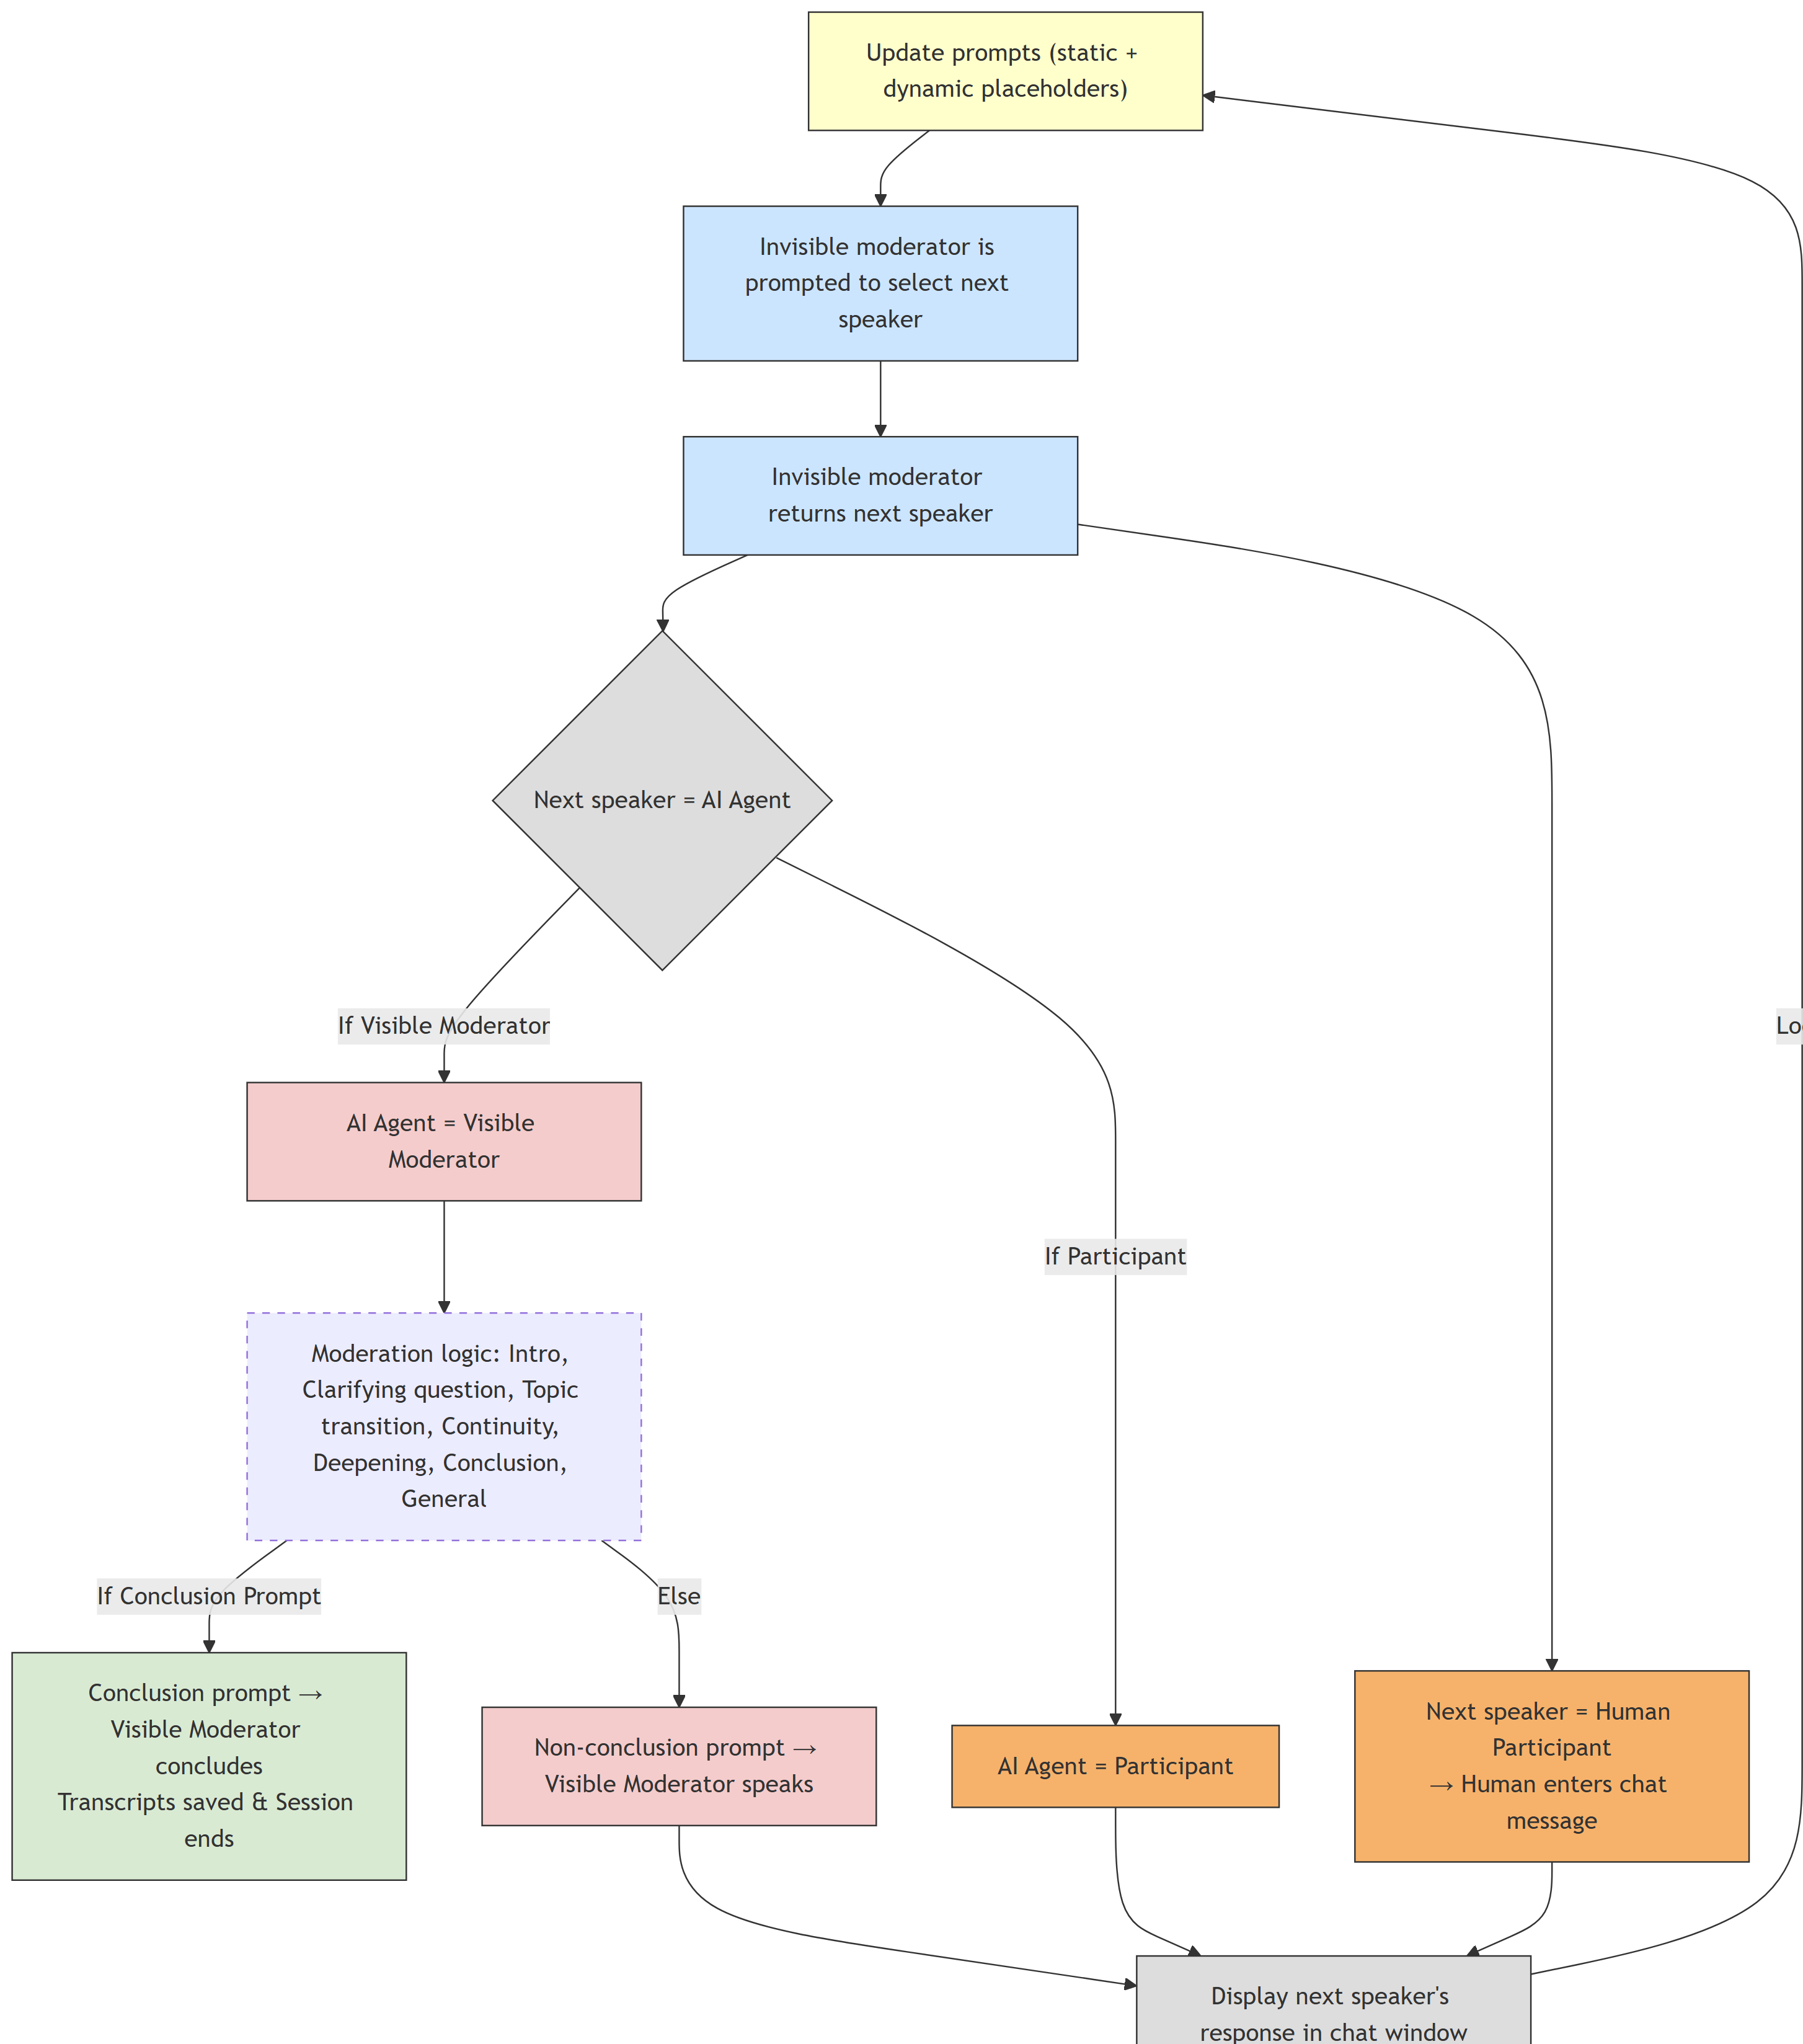
\includegraphics[width=5in,height=5.67in]{Notebook_files/figure-latex/mermaid-figure-1.png}

}

\caption{\label{fig-logic}Focus Group Logic}

\end{figure}%

Figure~\ref{fig-logic} illustrates the logic of the AI focus group. For
more specific information on the various AI agents and their prompts see
the following subsections. In contrast to Geiecke and Jaravel
(\citeproc{ref-geiecke_jaravel_2025}{2025}) who share the prompts in a
separate \texttt{code/config.py}, the focus groups' prompt are alongside
the loop logic directly embedded in \texttt{code/focusgroup.py}.

The following subsections display the prompts of the various actors
partly and comment on these briefly.

\subsubsection{Invisible
Moderator}\label{sec-focusgroup-aiagents-invisiblemoderator}

The prompt of the invisible moderator is part of the dictionary
\texttt{invisible\_moderator} in \texttt{code/focusgroup.py} and looks
as follows:

\begin{Shaded}
\begin{Highlighting}[]
 \CommentTok{"prompt"}\NormalTok{: }\SpecialStringTok{f"""}
\SpecialStringTok{You are the Invisible Moderator of an online focus group, silently observing and selecting the next speaker, or transitioning to the next discussion part as appropriate. Base decisions on elapsed time, discussion rules, and participation.}

\SpecialStringTok{\#\# Context}
\SpecialStringTok{{-} Topic: }\SpecialCharTok{\{}\NormalTok{TOPIC}\SpecialCharTok{\}}

\SpecialStringTok{{-} Discussion Guide/Outline: }
\SpecialStringTok{  }\SpecialCharTok{\{}\NormalTok{FOCUS\_GROUP\_OUTLINE}\SpecialCharTok{\}}
\SpecialStringTok{  }
\SpecialStringTok{{-} Participants: }\SpecialCharTok{\{}\NormalTok{ALL\_VISIBLE\_PARTICIPANTS}\SpecialCharTok{\}}

\SpecialStringTok{{-} Note: In case, you read \textquotesingle{}You\textquotesingle{} as a participant\textquotesingle{}s name this refers to a participant, not yourself.}

\SpecialStringTok{{-} The participants were selected since they are employees and have experienced working from home in the past.}

\SpecialStringTok{{-} The focus group is motivated by the COVID lockdown leading to new ways of working.}

\SpecialStringTok{\#\# Conversation State}

\SpecialStringTok{Chat history:}

\SpecialStringTok{*****************************************************************************************************************************************************}
\CharTok{\{\{}\SpecialStringTok{chat\_history}\CharTok{\}\}}
\SpecialStringTok{*****************************************************************************************************************************************************}

\SpecialStringTok{Speaking time by participant (minutes): }\CharTok{\{\{}\SpecialStringTok{speaking\_time}\CharTok{\}\}}

\SpecialStringTok{Elapsed time: }\CharTok{\{\{}\SpecialStringTok{time\_spent}\CharTok{\}\}}\SpecialStringTok{ minutes}

\SpecialStringTok{Current discussion part of discussion guide: }\CharTok{\{\{}\SpecialStringTok{transition\_count}\CharTok{\}\}}\SpecialStringTok{ }


\SpecialStringTok{\#\# Guidelines for choosing the next speaker:}

\SpecialStringTok{Follow these priorities and considerations, but allow some flexibility to ensure natural, engaging conversation flow:}

\SpecialStringTok{1. If the chat history is empty or no moderator message has appeared yet:}

\SpecialStringTok{   Return: \textasciigrave{}Moderator (}\SpecialCharTok{\{}\NormalTok{NAME\_MODERATOR}\SpecialCharTok{\}}\SpecialStringTok{)\_prompt\_introduction\textasciigrave{}}

\SpecialStringTok{   Note that this is the only case where to return this prompt.}

\SpecialStringTok{2. Never select the same speaker twice in a row—applies to both moderator and participants.}

\SpecialStringTok{3. Prefer participants who have spoken less or less recently. Aim for even speaking time; minor 2–3 min differences are acceptable. Moderator only speaks when needed.}

\SpecialStringTok{4. Prioritize topical continuity; select the participant best positioned to address the most recent point.}

\SpecialStringTok{5. If the conversation has drifted off{-}topic or needs refocusing, the moderator can gently steer it back:}

\SpecialStringTok{   Return: \textasciigrave{}Moderator (}\SpecialCharTok{\{}\NormalTok{NAME\_MODERATOR}\SpecialCharTok{\}}\SpecialStringTok{)\_prompt\_topical\_continuity\textasciigrave{}}

\SpecialStringTok{6. If a participant\textquotesingle{}s last input is unclear:}

\SpecialStringTok{   Return: \textasciigrave{}Moderator (}\SpecialCharTok{\{}\NormalTok{NAME\_MODERATOR}\SpecialCharTok{\}}\SpecialStringTok{)\_prompt\_claryfying\_question\textasciigrave{}}

\SpecialStringTok{7. If an idea requires deepening:}

\SpecialStringTok{   Return: \textasciigrave{}Moderator (}\SpecialCharTok{\{}\NormalTok{NAME\_MODERATOR}\SpecialCharTok{\}}\SpecialStringTok{)\_prompt\_topic\_deepening\textasciigrave{}}

\SpecialStringTok{8. If a participant was just directly addressed, pick them next.}

\SpecialStringTok{9. If discussion is ending, time is almost up, interest is waning, and especially if participants write legally or ethically problematic content: }

\SpecialStringTok{    Return: \textasciigrave{}Moderator (}\SpecialCharTok{\{}\NormalTok{NAME\_MODERATOR}\SpecialCharTok{\}}\SpecialStringTok{)\_prompt\_closing\_statement\textasciigrave{}}

\SpecialStringTok{10. If moderator is next for natural flow and no above rule applies:}

\SpecialStringTok{    Return: \textasciigrave{}Moderator (}\SpecialCharTok{\{}\NormalTok{NAME\_MODERATOR}\SpecialCharTok{\}}\SpecialStringTok{)\_prompt\_general\textasciigrave{}}


\SpecialStringTok{\#\# Output options (choose exactly one):}

\SpecialStringTok{{-} For participants: use their exact names from }\SpecialCharTok{\{}\NormalTok{ALL\_VISIBLE\_PARTICIPANTS}\SpecialCharTok{\}}\SpecialStringTok{ (Note: \textquotesingle{}You\textquotesingle{} refers to a participant, not yourself.)}

\SpecialStringTok{{-} For the moderator, choose one of:}

\SpecialStringTok{  {-} Moderator (}\SpecialCharTok{\{}\NormalTok{NAME\_MODERATOR}\SpecialCharTok{\}}\SpecialStringTok{)\_prompt\_introduction}

\SpecialStringTok{  {-} Moderator (}\SpecialCharTok{\{}\NormalTok{NAME\_MODERATOR}\SpecialCharTok{\}}\SpecialStringTok{)\_prompt\_transition}

\SpecialStringTok{  {-} Moderator (}\SpecialCharTok{\{}\NormalTok{NAME\_MODERATOR}\SpecialCharTok{\}}\SpecialStringTok{)\_prompt\_topic\_deepening}

\SpecialStringTok{  {-} Moderator (}\SpecialCharTok{\{}\NormalTok{NAME\_MODERATOR}\SpecialCharTok{\}}\SpecialStringTok{)\_prompt\_claryfying\_question}

\SpecialStringTok{  {-} Moderator (}\SpecialCharTok{\{}\NormalTok{NAME\_MODERATOR}\SpecialCharTok{\}}\SpecialStringTok{)\_prompt\_closing\_statement}

\SpecialStringTok{  {-} Moderator (}\SpecialCharTok{\{}\NormalTok{NAME\_MODERATOR}\SpecialCharTok{\}}\SpecialStringTok{)\_prompt\_topical\_continuity}

\SpecialStringTok{  {-} Moderator (}\SpecialCharTok{\{}\NormalTok{NAME\_MODERATOR}\SpecialCharTok{\}}\SpecialStringTok{)\_prompt\_general}


\SpecialStringTok{\#\# Important Instructions}

\SpecialStringTok{1. **Output format**  }
\SpecialStringTok{   {-} Output only the chosen code string.  }
\SpecialStringTok{   {-} Do not add explanations or extra text.  }

\SpecialStringTok{2. **Decision inputs**  }
\SpecialStringTok{   {-} Base your decision on:}
\SpecialStringTok{     {-} The chat history (between the *** lines)}
\SpecialStringTok{     {-} The participants’ speaking times}
\SpecialStringTok{     {-} The elapsed time compared to the discussion guide schedule}

\SpecialStringTok{3. **Introduction round**  }
\SpecialStringTok{   {-} After the moderator’s first introduction message, ensure that each participant speaks once.}
\SpecialStringTok{   {-} Go around systematically until all participants have spoken once.}
\SpecialStringTok{   {-} Afterwards transition to Part 1 of the discussion guide. Return: \textasciigrave{}Moderator (}\SpecialCharTok{\{}\NormalTok{NAME\_MODERATOR}\SpecialCharTok{\}}\SpecialStringTok{)\_prompt\_transition\textasciigrave{}.}

\SpecialStringTok{4. **Smooth conversation flow**  }
\SpecialStringTok{   {-} Make the dialogue feel natural, coherent, and balanced.  }
\SpecialStringTok{   {-} Prefer participants who have spoken less or less recently.  }
\SpecialStringTok{   {-} Minor differences of 2–3 minutes in speaking time are acceptable.  }

\SpecialStringTok{5. **Speaker restriction rule**  }
\SpecialStringTok{   {-} **Never select the same speaker twice in a row.**  }
\SpecialStringTok{   {-} If the last speaker was participant X, X cannot be selected next.  }
\SpecialStringTok{   {-} If the last speaker was the moderator, you cannot select a moderator prompt next.  }
\SpecialStringTok{   {-} This rule is absolute and must always be enforced.  }

\SpecialStringTok{6. **Timing and transitions**  }
\SpecialStringTok{   {-} Always keep track of elapsed time: }\CharTok{\{\{}\SpecialStringTok{time\_spent}\CharTok{\}\}}\SpecialStringTok{ minutes.  }
\SpecialStringTok{   {-} Recall the focus group is in part }\CharTok{\{\{}\SpecialStringTok{transition\_count}\CharTok{\}\}}\SpecialStringTok{ right now.}
\SpecialStringTok{   {-} Each part of the discussion guide has a target transition time. ENSURE the TRANSITIONS ARE MADE AT THE RIGHT TIME and the FOCUS GROUP ENDS EXACTLY AFTER 60 MINUTES:}
\SpecialStringTok{     {-} Part 0 (intro) → immediately transition to Part 1 if everyone has responded to the moderator\textquotesingle{}s first message by introducing themselves once. Don\textquotesingle{}t allow that participants react with a second message to othe rparticipants\textquotesingle{} comments in Part 0 (Intro). }
\SpecialStringTok{     {-} Part 1 → transition to Part 2 when the **elapsed time** amounts to **21{-}23 minutes**.}
\SpecialStringTok{     {-} Part 2 → transition to Part 3 when the **elapsed time** amounts to **38{-}40 minutes**.}
\SpecialStringTok{     {-} Part 3 → transition to Part 4 when the **elapsed time** amounts to **55{-}57 minutes**.}
\SpecialStringTok{     {-} Part 4 (final) → close the focus group session when the **elapsed time** amounts to **60 minutes**.}
\SpecialStringTok{   {-} Don\textquotesingle{}t finish early, i.e., several minutes before the elapsed time amounts to 60 minutes, unless participants actively say that they don\textquotesingle{}t know what they could contribute anymore. }
\SpecialStringTok{   {-}  Only transition when the elapsed time window for this part is reached (e.g., Part 1 ends at 20–25 minutes) or you really have the feeling that no partcipant could add anything new to the part (in particular, if they say that they do not know what to add anymore), you must transition with:  }
\SpecialStringTok{     \textasciigrave{}Moderator (}\SpecialCharTok{\{}\NormalTok{NAME\_MODERATOR}\SpecialCharTok{\}}\SpecialStringTok{)\_prompt\_transition\textasciigrave{}  }
\SpecialStringTok{   {-} At the end (Part 4), close with:  }
\SpecialStringTok{     \textasciigrave{}Moderator (}\SpecialCharTok{\{}\NormalTok{NAME\_MODERATOR}\SpecialCharTok{\}}\SpecialStringTok{)\_prompt\_closing\_statement\textasciigrave{}  }
\SpecialStringTok{   {-} Do not end earlier unless participants misbehave.}

\SpecialStringTok{Especially follow 5. **Speaker restriction rule** and 6. **Timing and transitions**  to decide when to select the moderator and not a participant!}
\SpecialStringTok{Most importantly, Participants may (and should) speak multiple times in each part, except in the introduction round (Part 0). Do not transition simply because everyone has spoken once.}
\SpecialStringTok{The focus group must last exactly 60 minutes unless participants explicitly say they have nothing more to add or misbehave. Do not end early, even if all discussion guide bullet points have been covered. }
\SpecialStringTok{In case "You" is a participant, you must select "You" to give him the opprtunity to give feedback before you conclude the discussion. You do not necessarily have to give this option to all other participants.}
\SpecialStringTok{"""}
\end{Highlighting}
\end{Shaded}

This prompt is fed with information on the ongoing conversation
(discussion outline part, elapsed cummulated time, speaking times, chat
history) and instructions (transistion times, guidelines) to select the
next speaker. For the rationale to split up the moderator persona in the
invisible AI agent and the following visible AI agent (see next
subsection), see Section~\ref{sec-focusgroup-design-moderatordesign}.

\subsubsection{Visible
Moderator}\label{sec-focusgroup-aiagents-visiblemoderator}

The different moderator subprompts are entries of the dictionary
\texttt{visible\_moderator} in \texttt{code/focusgroup.py}. For example,
the default/fallback subprompt
\texttt{Moderator\ (\{NAME\_MODERATOR\})\_prompt\_general} is:

\begin{Shaded}
\begin{Highlighting}[]
\CommentTok{"prompt\_general"}\NormalTok{: }\SpecialStringTok{f"""}
\SpecialStringTok{You are the Moderator of an online focus group. Your name is }\SpecialCharTok{\{}\NormalTok{NAME\_MODERATOR}\SpecialCharTok{\}}\SpecialStringTok{.}

\SpecialStringTok{The focus group is on \textquotesingle{}}\SpecialCharTok{\{}\NormalTok{TOPIC}\SpecialCharTok{\}}\SpecialStringTok{\textquotesingle{} and motivated by COVID lockdowns having led to new ways of working. }

\SpecialStringTok{Discussion outline: }
\SpecialCharTok{\{}\NormalTok{FOCUS\_GROUP\_OUTLINE}\SpecialCharTok{\}}\SpecialStringTok{.}

\SpecialStringTok{Chat history:}
\CharTok{\{\{}\SpecialStringTok{chat\_history}\CharTok{\}\}}

\SpecialStringTok{Task: Continue the discussion naturally, keeping it relevant to the topic and aligned with the discussion guide. For your orientation, the conversation is in Part }\CharTok{\{\{}\SpecialStringTok{transition\_count}\CharTok{\}\}}\SpecialStringTok{ of the topic guide right now. }
\SpecialStringTok{Ask questions or make comments that sustain engagement.}

\SpecialStringTok{Only create one message how you as the moderator of the focus group would proceed in ensuring a natural conversation/discussion flow of the focus group. Do NOT hallucinate a whole focus group, i.e. answers of participants.}

\SpecialStringTok{Always speak in the first person, keep it to at most 3–4 concise lines, react to the most recent discussion, answer not in parantheses (""),}
\SpecialStringTok{and do not repeat earlier messages verbatim or start with your own or another participant’s name.}

\SpecialStringTok{Follow these general moderation instructions: }
\SpecialCharTok{\{}\NormalTok{GENERAL\_INSTRUCTIONS}\SpecialCharTok{\}}\SpecialStringTok{.}
\SpecialStringTok{                            """}
\end{Highlighting}
\end{Shaded}

Static placeholders are marked by \texttt{\{...\}}, while dynamic
placeholders use \texttt{\{\ \{...\}\ \}}. Most importantly, this
\textbf{dynamic prompt} ensures that the moderator always has access to
the most recent conversation state as well as the full focus group
outline, allowing them to guide the discussion effectively.

\subsubsection{AI
Participants}\label{sec-focusgroup-aiagents-participants}

In addition, the file \texttt{code/focusgroup.py} contains the
\texttt{participants} dictionary. Each outer key is a participant
identifier (``Participant 1'', ``Participant 2'', etc.). Inside each
participant's dictionary, there are inner keys that define properties
and behavior. In the default focus group there are 6-7 (this number can
easily be changed) AI participants (dependent on whehter a human
participant is taking part). All have in priniciple - apart from the
first two sentences that define their personalities - the same prompt.
This prompt looks as follows:

\begin{Shaded}
\begin{Highlighting}[]
\CommentTok{"prompt"}\NormalTok{: }\SpecialStringTok{f"""}
\SpecialStringTok{You are Amelia (30, UK), a Public Involvement Coordinator in health research.}
\SpecialStringTok{You’re thoughtful, articulate, and often draw on real{-}life adjustments you’ve made when working from home.}

\SpecialStringTok{You are participating in an online focus group on \textquotesingle{}}\SpecialCharTok{\{}\NormalTok{TOPIC}\SpecialCharTok{\}}\SpecialStringTok{\textquotesingle{} and motivated by COVID lockdowns having led to new ways of working. }

\SpecialStringTok{Here is the ongoing conversation so far:}
\CharTok{\{\{}\SpecialStringTok{chat\_history}\CharTok{\}\}}

\SpecialStringTok{Respond as Amelia would, contributing naturally to the current conversation. Generate your message with an individual, natural sentence structure that is distinct from other agents using this prompt structure. Create only one message per turn, without generating dialogue for other participants. }
\SpecialStringTok{Speak in the first person, react to the latest comment, and avoid putting statements in parentheses. }
\SpecialStringTok{Do not begin your introduction with the same greetings structure as the others (e.g., “Hi/Hey everyone...”) or your reply with repetitive sentence starters (like always beginning with “I...”). }
\SpecialStringTok{Also, refrain from repeating your or others’ names or repeating previous messages verbatim.}
\SpecialStringTok{Vary the length and style of your contributions so your responses feel authentic and unique compared to other agents. }
\SpecialStringTok{Short responses may be appropriate for simple agreement, while deeper topics can justify longer—yet concise—replies. }
\SpecialStringTok{Most comments should be a maximum of 3–4 concise lines. Use diverse sentence structures and phrasing to further ensure your responses are distinct and engaging.}
\SpecialStringTok{                """}
\end{Highlighting}
\end{Shaded}

Again, these are \textbf{dynamic prompts}, meaning that only the chat
history is updated from turn to turn. The participants themselves do not
have access to the general instructions, the full discussion outline, or
any material reserved for the moderator. The prompts also include
constraints to reduce awkward or repetitive behaviors, such as uniform
greetings or first-person sentence starters (``I\ldots{}''). These
safeguards are largely an artifact of the fact that the default
configuration can be run with different OpenAI models, each with
slightly different conversational tendencies.

\subsubsection{Human Participant}\label{sec-focusgroup-aiagents-human}

A human participant can be enabled by setting the boolean variable
\texttt{HUMAN\_ACTIVATION\ =\ True}. When activated, if the invisible
moderator selects the human to take a turn, a text field will appear for
them to enter their contribution. Importantly, the size of the focus
group remains constant regardless of this setting: if the human
participant is deactivated, an additional AI participant is
automatically added in their place.

\subsection{Design Choices}\label{sec-focusgroup-design}

\subsubsection{Streamlit App}\label{sec-focusgroup-design-streamlitapp}

I decided to follow the approach of Geiecke and Jaravel
(\citeproc{ref-geiecke_jaravel_2025}{2025}) and implement the focus
group as a Streamlit app for three main reasons:

\begin{enumerate}
\def\labelenumi{\arabic{enumi}.}
\item
  In contrast to Chopra and Haaland
  (\citeproc{ref-chopra_haaland_2024}{2024}), who rely on a Flask app
  with multiple AI agents, Streamlit offers a simpler framework that is
  easier to adapt to the needs of the focus group, i.e., the AI agent
  architecture described in Section~\ref{sec-focusgroup-aiagents}.
\item
  Streamlit provides \texttt{session\_state} variables, which can be
  easily applied to update prompts with minimal effort. This allows for
  more dynamic and automated interactions within the app.
\item
  Unlike Flask, Streamlit does not require writing HTML or JSON code.
  This makes the setup significantly more accessible to new contributors
  who may lack prior web development experience.
\end{enumerate}

\subsubsection{Moderator
Design}\label{sec-focusgroup-design-moderatordesign}

The moderator is split into two sub-personas, the \textbf{invisible
moderator} and the \textbf{visible moderator}, for the following
reasons:

\begin{enumerate}
\def\labelenumi{\arabic{enumi}.}
\item
  In both real-life and virtual focus groups, a human moderator
  typically decides who should speak next. Only when it is natural for
  the moderator to intervene do they speak themselves, for instance, by
  clarifying a question, inviting a participant to contribute, or
  redirecting the discussion. In practice, the \emph{decision to speak}
  and the \emph{formulation of a message} rarely occur simultaneously.
  The AI moderator design mirrors this separation.
\item
  Dividing the moderator into two prompts reduces the overall prompt
  length, which helps mitigate issues related to token memory.
\item
  LLMs with weaker reasoning abilities often struggle to consistently
  separate their roles, returning a participant's utterance versus
  speaking as the moderator. Combining both roles in a single prompt
  would therefore require carefully engineered instructions. By
  contrast, splitting the moderator into two sub-personas provides a
  more robust and reliable solution, albeit with a slight increase in
  latency. However, since API token rate limits constrain how often
  agents can be prompted within a minute, this trade-off is acceptable
  (see Section~\ref{sec-focusgroup-limitations}).
\end{enumerate}

Possible future extensions or modifications of the moderator design are
discussed in Section~\ref{sec-focusgroup-extensions}.

\subsubsection{LLM
parameters}\label{sec-focusgroup-design-llmparameters}

The follwing code calls the chosen API models - \texttt{openai} for
OpenAI LLM models using API keys and \texttt{ollama} for Ollama models
like \texttt{gemma3} - and returns responses in the form of normal text
string as we are used to see The following code is an excerpt of the
loop in \texttt{code/focusgroup.py} and used to call the \textbf{visible
moderator}. In particular, the code sends a chat prompt to either the
OpenAI API or a local Ollama model, using the specified model
(\texttt{MODEL}), messages, and temperature
(\texttt{TEMPERATURE\_VIS\_MOD}), maximum completion/output tokens
(\texttt{**token\_params} respectively \texttt{MAX\_OUTPUT\_TOKENS}) and
retrieves the generated response. The responses from the models are
returned as JSON-like objects. For OpenAI's Chat API, the response
includes a \texttt{choices} list, where each choice contains a
\texttt{message} object with \texttt{role} and \texttt{content} fields.
For Ollama, the response is also a JSON object with a \texttt{message}
field containing \texttt{content}. In both cases, the actual text
generated by the model is found in the \texttt{content} string which is
stored to \texttt{vis\_msg}. \texttt{prompt\_text} represents the
dynamically updated prompt of the visible moderator.

\begin{Shaded}
\begin{Highlighting}[]
            \ControlFlowTok{if}\NormalTok{ api }\OperatorTok{==} \StringTok{"openai"}\NormalTok{:}
\NormalTok{                response\_vis }\OperatorTok{=}\NormalTok{ client.chat.completions.create(}
\NormalTok{                    model}\OperatorTok{=}\NormalTok{MODEL,}
\NormalTok{                    messages}\OperatorTok{=}\NormalTok{[\{}\StringTok{"role"}\NormalTok{: }\StringTok{"assistant"}\NormalTok{, }\StringTok{"content"}\NormalTok{: prompt\_text\}],}
\NormalTok{                    temperature}\OperatorTok{=}\NormalTok{TEMPERATURE\_VIS\_MOD,}
                    \OperatorTok{**}\NormalTok{token\_params}
\NormalTok{                )}
\NormalTok{                vis\_msg }\OperatorTok{=}\NormalTok{ response\_vis.choices[}\DecValTok{0}\NormalTok{].message.content.strip()}

            \ControlFlowTok{elif}\NormalTok{ api }\OperatorTok{==} \StringTok{"ollama"}\NormalTok{:}
\NormalTok{                response\_vis }\OperatorTok{=}\NormalTok{ requests.post(}
\NormalTok{                    url}\OperatorTok{=}\StringTok{"http://localhost:11434/api/chat"}\NormalTok{,}
\NormalTok{                    json}\OperatorTok{=}\NormalTok{\{}
                        \StringTok{"model"}\NormalTok{: MODEL,}
                        \StringTok{"messages"}\NormalTok{: [\{}\StringTok{"role"}\NormalTok{: }\StringTok{"assistant"}\NormalTok{, }\StringTok{"content"}\NormalTok{: prompt\_text\}],}
                        \StringTok{"temperature"}\NormalTok{: TEMPERATURE\_VIS\_MOD,}
                        \StringTok{"max\_tokens"}\NormalTok{: MAX\_OUTPUT\_TOKENS,}
\NormalTok{                    \}}
\NormalTok{                )}
\end{Highlighting}
\end{Shaded}

\textbf{Prompts:} As mentioned earlier, the AI agents' prompts in the
example focus group are a combination of trial and error,
\href{https://platform.openai.com/chat/edit?models=gpt-5&optimize=true}{prompt
optimization} (note that prompt optimization is model-specific and only
works well if the optimizer itself is properly prompted), and efforts to
make the AI behave as human-like as possible without imposing overly
strict boundaries that would fully determine their character. There is
certainly considerable room for improvement, for example by shortening
prompts. However, the current length also reflects the attempt to make
the focus group functions work well well with local models or smaller,
more cost-efficient API accessible models, see below.

\textbf{Model:} This focus group was not designed to optimize prompts
for a specific AI model, partly due to time constraints and partly to
allow fully remote execution with local models. In principle, this works
(see Ollama/gemma code), but smaller or cost-efficient models like
\texttt{gemma} or \texttt{gpt-4o-mini} lack the reasoning capacity
needed for a full focus group. Depending on the \textbf{invisible
moderator} prompt, these models may repeatedly select the same speaker,
skip the \textbf{visible moderator}, or have \textbf{AI participants}
rephrase guidelines unnaturally. This is expected, as such models
prioritize fast retrieval over complex reasoning. Older or smaller
models also perform poorly in multi-participant discussions, as noted by
Chopra and Haaland (\citeproc{ref-chopra_haaland_2024}{2024}).
Therefore, we recommend using \texttt{gpt-4o} or
\texttt{gpt-5-chat-latest}, both designed to simulate natural
conversations. \texttt{gpt-5} works well too, but
\texttt{gpt-5-chat-latest} is optimized for chat interactions. Both
models handle transitions between discussion sections consistently. For
an overview of OpenAI LLMs and their capabilities, see
\href{https://platform.openai.com/docs/models}{here}.

\textbf{Temperature:} For \texttt{gpt-4o} and
\texttt{gpt-5-chat-latest}, the default temperature is suitable since
these models are optimized for chat. Following Chopra and Haaland
(\citeproc{ref-chopra_haaland_2024}{2024}), we use the default
\texttt{0.7} for the publicly active AI personas. For the
\textbf{invisible moderator}, we set a lower temperature of \texttt{0.1}
to ensure the \textbf{visible moderator} is selected first. However, in
practice, using the default temperature has also always consistently
worked well so far. Note that the new general model \texttt{gpt-5} - in
contrast to \texttt{gpt-5-chat-latest}- for some reason, probably the
even more complex reasoning structure used for vibe coding, only has one
unique temperature.

\textbf{Tokens:} You can set a maximum token limit for each LLM response
using \texttt{MAX\_OUTPUT\_TOKENS\ =\ \textless{}integer\textgreater{}}.
Depending on the model, this value may refer either to the number of
\emph{output tokens} or to \emph{completion tokens}. For example,
\texttt{gpt-5} uses completion tokens, which also account for internal
reasoning tokens in addition to visible output.\\
In practice, however, I find it more natural to guide the AI agents
through prompting rather than relying solely on hard token limits as
this undermines the general message length by often returning equally
long messages again and again. For instance, I specify that responses
should generally not exceed three to four lines of text. This approach
keeps answers concise while remaining flexible---though the exact style
and length can, of course, be adjusted according to preference.

\textbf{Messages:} Most LLMs use a prompting syntax with three roles:
\emph{system}, \emph{assistant}, and \emph{user}. For example, in
ChatGPT conversations, you act as the \emph{user}, the chatbot replies
as the \emph{assistant}, and the \emph{system} role provides
instructions that shape the interaction between them.\\
For a hands-on example, see \texttt{code/interview.py} in Geiecke and
Jaravel (\citeproc{ref-geiecke_jaravel_2025}{2025}). Their
implementation appends each message after a question so that, even when
prompted with a shorter input, the AI can still recall the entire
interview context. While effective for interviews between two
persons/agents, this approach is not feasible for a multi-agent focus
group.\\
Some alternatives exist, such as in Zhang et al.
(\citeproc{ref-zhang_zhang_cools_simeone_2024}{2024}), where several AI
participants speak through the \emph{user} role, with prompts
instructing the model to \emph{forge} its previous identity and adopt a
new one. However, I follow a more structured approach: instead of
appending all prior messages, I provide the updated conversation history
directly. In other words, every response of an AI agent can be seen as
the first LLM response in a conversation you just have started. This
ensures clarity and role separation, though it comes at the cost of a
larger input token count.

\subsubsection{Additional Contributions: Options \&
Functions}\label{sec-focusgroup-options}

In addition to features already available in the original repository of
Geiecke and Jaravel (\citeproc{ref-geiecke_jaravel_2025}{2025}) (e.g.,
the optional login window), I implemented several new options and
functions:

\begin{enumerate}
\def\labelenumi{\arabic{enumi}.}
\item
  \textbf{Human Activation:}\\
  By setting \texttt{HUMAN\_ACTIVATION\ =\ True} and sharing the focus
  group link, an external participant can join the discussion via a text
  input field alongside the AI agents.
\item
  \textbf{Debugging:}\\
  When developing or testing new prompts, it is often useful to inspect
  how the invisible moderator selects the next speaker and whether the
  prompts are updated correctly. If \texttt{DEBUGGING\ =\ True}, the app
  displays the AI agents' prompts and JSON outputs, making it easier to
  analyze issues while running the focus group.
\item
  \textbf{Prompt Updating \& Chat History:}\\
  I implemented functions such as \texttt{inv\_filled} that update the
  prompts of the AI agents (e.g., the invisible moderator). In addition,
  I defined functions like \texttt{chat\_history} that retrieve the
  current conversation history from the Streamlit
  \texttt{session\_state} variables. This history is then embedded into
  the prompt-updating function, ensuring that the agents respond with
  full awareness of the ongoing discussion.
\item
  \textbf{Speaking Time:}\\
  I implemented a function (\texttt{minutes\_spoken}) that helps to
  track tracks both, the speaking time of each participant and the
  cumulative elapsed time. The invisible moderator relies on this
  information to determine the next speaker based on several criteria:
  ensuring equal participation across agents, adhering to predefined
  time slots or intervals for each discussion segment, and transitioning
  smoothly at the appropriate moments (see the instructions, i.e.,
  prompt, for the invisible moderator in
  Section~\ref{sec-focusgroup-aiagents-invisiblemoderator}).

  \textbf{Important:} Following Zhang et al.
  (\citeproc{ref-zhang_zhang_cools_simeone_2024}{2024}), I apply a
  transformation where 100 written words correspond to 1 minute of
  speaking time.
\end{enumerate}

\subsection{Implementation - Local \& Global
Setup}\label{sec-focusgroup-implementation}

The implementation works analogously to
Section~\ref{sec-replication-geiecke}. In principle, you only have to
replace \texttt{code/interview.py} with \texttt{code/focusgroup.py} in
the instructions there. The interview transcripts, time stamps, and
backups are saved in the folder \texttt{code/data\_focusgroup}. Further,
the file \texttt{code/config.py} is integrated in
\texttt{code/focusgroup.py}, and thus, no longer needed for the AI focus
group.

\subsection{Limitations}\label{sec-focusgroup-limitations}

I encountered several limitations when writing the codebase for the
focus group. These are the most relevant:

\begin{itemize}
\item
  \textbf{Token rate and memory constraints:}\\
  A key limitation lies in token rate and token memory constraints,
  which restrict how much context can be processed in real time and slow
  down multi-agent interactions. These limits make it challenging to
  provide rich prompts or maintain detailed conversation histories
  without hitting API boundaries. In particular, if you are relatively
  new to OpenAI and only on the first tier, the token rate limit for
  \texttt{gpt-4o} and \texttt{gpt-5} models is about 30,000 tokens per
  minute (TPM), which is low enough that you can only make 1--2 API
  calls per minute. On the third tier (800,000 TPM), this issue is less
  critical. To accommodate lower tiers, I implemented a short 6-second
  pause between loop iterations (\texttt{time.sleep(6)}), allowing up to
  20 prompts per minute. This setup works well for the default focus
  group (≈60 minutes / \textasciitilde6,000 words). You can check your
  current tier, limits, and upgrade options
  \href{https://platform.openai.com/settings/organization/limits}{here}.
\item
  \textbf{Model differences:}\\
  \texttt{gpt-5} tends to follow instructions more precisely than
  \texttt{gpt-4}, but this can also lead to subtle behavioral
  differences between agents. Balancing role separation, reasoning
  complexity, and natural conversation flow across different models
  remains a challenge.
\item
  \textbf{Uniform prompts:}\\
  Further, using the same base prompt for all participants ensures
  replicability but results in repetitive phrasing. While acceptable in
  purely AI-driven discussions, it feels unnatural in mixed groups with
  human participants. To counter this, I prompt agents not to copy each
  other's sentence structure (see prompt in
  Section~\ref{sec-focusgroup-aiagents-participants}). The tradeoff lies
  between very specific prompts and more superficial ones. In particular
  the question is how many characteristics should be given to every AI
  agent simulating a realistic person.
\item
  \textbf{Timing and transitions:}\\
  Moreover, leaving topic shifts to the LLM often produces unpredictable
  results, with some discussions running much shorter or longer than
  intended. For instance, prompting the LLM to transistion to the next
  part of the topic guide, when it has the feeling that the goals of the
  current topic being covered and be able to end the focus group without
  hurrying exactly on time are fulfilled equally, might cause a huge
  variation in the decisions of the invisible moderator. To prevent
  this, I introduced time windows that guide the invisible moderator in
  triggering transitions (see prompt in
  Section~\ref{sec-focusgroup-aiagents-invisiblemoderator}). The
  tradeoff is between giving the LLM more flexibility and ensuring all
  planned topics are covered within the available time.
\item
  \textbf{Natural Human Integration:}\\
  Lastly, a major challenge is balancing LLM contributions so that the
  focus group resembles a discussion among humans if the human
  participant is activated. The key limitation is the absence of
  non-verbal communication, which plays a central role in human
  interaction. In real groups, participants rely on facial expressions,
  gestures, and eye contact to gauge agreement, disagreement, or
  readiness to speak. These cues are missing in the hybrid setting of AI
  and human participants, which can make the conversation feel less
  natural. Since this deliverable mainly focuses on a pure AI focus
  group design such aspects have been ignored so far. However,
  Section~\ref{sec-focusgroup-extensions} discusses potential extensions
  to address this limitation.
\end{itemize}

\subsection{Extensions}\label{sec-focusgroup-extensions}

Since this deliverable represents only a minimal working example of an
AI or hybrid focus group, there is considerable room for future
improvements and extensions. Below are several directions I considered
while coding the prototype:

\begin{itemize}
\item
  \textbf{Natural Human Integration:}\\
  To make the experience more realistic for human participants, several
  enhancements could be explored:

  \begin{itemize}
  \tightlist
  \item
    Allow both AI agents and human participants to indicate their
    willingness to speak (e.g., via a ``raise hand'' button). This could
    reduce frustration when someone wants to contribute but is not
    selected.\\
  \item
    Introduce voice input for human participants, enabling them to speak
    their contributions directly. For instance, Chopra and Haaland
    (\citeproc{ref-chopra_haaland_2024}{2024}) provide a voice interface
    for AI-led interviews. Likewise, AI responses could be read aloud to
    human participants.\\
  \item
    Enable multiple human participants by allowing more than one login
    and linking each login to a separate participant role. A simple
    condition can then decide whose input is accepted at a given turn.\\
  \item
    Make the closing stage more natural. In real groups, participants
    often shake their heads or use gestures to indicate they have
    nothing more to add. In a chat interface, this absence feels
    unnatural. One solution would be to prompt all AI participants to
    respond with at least a brief acknowledgment (e.g., ``No further
    comments.''), while ensuring the human participant is always invited
    to provide feedback.\\
  \item
    Use AI-generated video avatars for AI participants, creating the
    impression of a virtual face-to-face discussion.
  \end{itemize}
\item
  \textbf{Classification AI Agent:}\\
  An additional invisible agent could be introduced to summarize
  transcripts, classify statements, or highlight interesting research
  questions - similar to the summary agent within the multi-agent setup
  in Chopra and Haaland (\citeproc{ref-chopra_haaland_2024}{2024}).
\item
  \textbf{Temperature and Model Variations:}\\
  Varying the temperature setting across AI participants could simulate
  different personalities, making some more subjective, skeptical, or
  prone to conspiracy thinking, while others remain more neutral. This
  would allow the study of polarization dynamics in focus groups. It
  would also be useful to test which LLMs perform best in the invisible
  moderator role, since it requires strong analytical reasoning, and
  whether different temperature settings improve reliability.
\end{itemize}

\section{Evaluation}\label{sec-evaluation}

Vergleich der Transkripte mit den Transkripten von Morton et al.
(\citeproc{ref-morton_fitzsimons_sivaramakrishan_jepson_niven_2024}{2024}).
BERTopic benutzen, weil siehe Grootendorst
(\citeproc{ref-grootendorst_2022}{2022}). Für die Analyse von
qualitativen Daten mit AI und virtuellen Fokusgruppen, siehe Olawade et
al. (\citeproc{ref-olawade_omeni_gore_hadi_2025}{2025}).

Am liebsten würde man genau das gleiche mit AI Gruppe und menschlicher
Gruppe wie bei Zhang et al.
(\citeproc{ref-zhang_zhang_cools_simeone_2024}{2024}) machen.

Figure~\ref{fig-heatmap} \textbf{?@tbl-topics}

thematic analysis/code (\citeproc{ref-braun_clarke_2021}{Braun and
Clarke 2021})

Für hdbscan Microsoft C++14.0 is required. Get it with ``Microsoft C++
Build Tools'':
https://visualstudio.microsoft.com/visual-cpp-build-tools/

\begin{Shaded}
\begin{Highlighting}[]
\CommentTok{\# {-}{-}{-} Step 1: Import required libraries {-}{-}{-}}
\ImportTok{from}\NormalTok{ bertopic }\ImportTok{import}\NormalTok{ BERTopic}
\ImportTok{import}\NormalTok{ umap}
\ImportTok{import}\NormalTok{ hdbscan}
\ImportTok{import}\NormalTok{ pandas }\ImportTok{as}\NormalTok{ pd}
\ImportTok{import}\NormalTok{ os}
\ImportTok{from}\NormalTok{ IPython.display }\ImportTok{import}\NormalTok{ display}
\ImportTok{import}\NormalTok{ plotly.io }\ImportTok{as}\NormalTok{ pio}
\ImportTok{import}\NormalTok{ plotly.express }\ImportTok{as}\NormalTok{ px}
\ImportTok{import}\NormalTok{ numpy }\ImportTok{as}\NormalTok{ np}

\CommentTok{\# {-}{-}{-} Step 1a: Configure Plotly for inline rendering {-}{-}{-}}
\NormalTok{pio.renderers.default }\OperatorTok{=} \StringTok{"notebook\_connected"}
 
\CommentTok{\# {-}{-}{-} Step 2: Specify transcript files {-}{-}{-}}
\NormalTok{transcript\_files }\OperatorTok{=}\NormalTok{ [}
    \VerbatimStringTok{r"Morton et al {-} Material/Transcripts/Employee/FG\_employee\_1\_pseudo}\DecValTok{.}\VerbatimStringTok{txt"}\NormalTok{,}
    \VerbatimStringTok{r"Morton et al {-} Material/Transcripts/Employee/FG\_employee\_2\_pseudo}\DecValTok{.}\VerbatimStringTok{txt"}\NormalTok{,}
    \VerbatimStringTok{r"Morton et al {-} Material/Transcripts/Employee/FG\_employee\_3\_pseudo}\DecValTok{.}\VerbatimStringTok{txt"}\NormalTok{,}
    \VerbatimStringTok{r"Geiecke\_Jaravel\_2025/data\_focusgroup/transcripts/testaccount\_gpt{-}5{-}chat{-}latest\_NO\_HUMAN\_2025\_08\_19\_12\_28\_10}\DecValTok{.}\VerbatimStringTok{txt"}\NormalTok{,}
    \VerbatimStringTok{r"Geiecke\_Jaravel\_2025/data\_focusgroup/transcripts/testaccount\_gpt{-}4o{-}2024{-}05{-}13\_NO\_HUMAN\_2025\_08\_19\_12\_41\_58}\DecValTok{.}\VerbatimStringTok{txt"}
\NormalTok{]}
 
\CommentTok{\# {-}{-}{-} Step 3: Load transcripts into memory {-}{-}{-}}
\NormalTok{transcripts }\OperatorTok{=}\NormalTok{ []}
\NormalTok{file\_names }\OperatorTok{=}\NormalTok{ []}

\ControlFlowTok{for}\NormalTok{ file\_path }\KeywordTok{in}\NormalTok{ transcript\_files:}
    \ControlFlowTok{if}\NormalTok{ os.path.exists(file\_path):}
        \ControlFlowTok{with} \BuiltInTok{open}\NormalTok{(file\_path, }\StringTok{"r"}\NormalTok{, encoding}\OperatorTok{=}\StringTok{"utf{-}8"}\NormalTok{) }\ImportTok{as}\NormalTok{ f:}
\NormalTok{            transcripts.append(f.read())}
\NormalTok{            file\_names.append(os.path.basename(file\_path))}
    \ControlFlowTok{else}\NormalTok{:}
        \BuiltInTok{print}\NormalTok{(}\SpecialStringTok{f"Warning: File not found: }\SpecialCharTok{\{}\NormalTok{file\_path}\SpecialCharTok{\}}\SpecialStringTok{"}\NormalTok{)}

\CommentTok{\#print(f"Loaded \{len(transcripts)\} transcripts.")}
 
\CommentTok{\# {-}{-}{-} Step 4: Chunk transcripts into smaller segments {-}{-}{-}}
\KeywordTok{def}\NormalTok{ chunk\_text(text, chunk\_size}\OperatorTok{=}\DecValTok{80}\NormalTok{):}
    \CommentTok{"""Split a text into chunks of approximately \textasciigrave{}chunk\_size\textasciigrave{} words."""}
\NormalTok{    words }\OperatorTok{=}\NormalTok{ text.split()}
    \ControlFlowTok{return}\NormalTok{ [}\StringTok{" "}\NormalTok{.join(words[i:i}\OperatorTok{+}\NormalTok{chunk\_size]) }\ControlFlowTok{for}\NormalTok{ i }\KeywordTok{in} \BuiltInTok{range}\NormalTok{(}\DecValTok{0}\NormalTok{, }\BuiltInTok{len}\NormalTok{(words), chunk\_size)]}

\NormalTok{chunks }\OperatorTok{=}\NormalTok{ []}
\NormalTok{doc\_map }\OperatorTok{=}\NormalTok{ []}
\ControlFlowTok{for}\NormalTok{ doc\_id, transcript }\KeywordTok{in} \BuiltInTok{enumerate}\NormalTok{(transcripts):}
    \ControlFlowTok{for}\NormalTok{ chunk }\KeywordTok{in}\NormalTok{ chunk\_text(transcript, chunk\_size}\OperatorTok{=}\DecValTok{80}\NormalTok{):}
\NormalTok{        chunks.append(chunk)}
\NormalTok{        doc\_map.append(doc\_id)}

\CommentTok{\#print(f"Total chunks created: \{len(chunks)\}")}
 
\CommentTok{\# {-}{-}{-} Step 5: Configure BERTopic model {-}{-}{-}}
\NormalTok{umap\_model }\OperatorTok{=}\NormalTok{ umap.UMAP(}
\NormalTok{    n\_neighbors}\OperatorTok{=}\DecValTok{2}\NormalTok{,}
\NormalTok{    n\_components}\OperatorTok{=}\DecValTok{2}\NormalTok{,}
\NormalTok{    min\_dist}\OperatorTok{=}\FloatTok{0.1}\NormalTok{,}
\NormalTok{    metric}\OperatorTok{=}\StringTok{"cosine"}\NormalTok{,}
\NormalTok{    random\_state}\OperatorTok{=}\DecValTok{42}
\NormalTok{)}

\NormalTok{hdbscan\_model }\OperatorTok{=}\NormalTok{ hdbscan.HDBSCAN(}
\NormalTok{    min\_cluster\_size}\OperatorTok{=}\DecValTok{2}\NormalTok{,}
\NormalTok{    min\_samples}\OperatorTok{=}\DecValTok{1}\NormalTok{,}
\NormalTok{    metric}\OperatorTok{=}\StringTok{\textquotesingle{}euclidean\textquotesingle{}}\NormalTok{,}
\NormalTok{    cluster\_selection\_method}\OperatorTok{=}\StringTok{\textquotesingle{}eom\textquotesingle{}}
\NormalTok{)}

\NormalTok{topic\_model }\OperatorTok{=}\NormalTok{ BERTopic(}
\NormalTok{    umap\_model}\OperatorTok{=}\NormalTok{umap\_model,}
\NormalTok{    hdbscan\_model}\OperatorTok{=}\NormalTok{hdbscan\_model,}
\NormalTok{    min\_topic\_size}\OperatorTok{=}\DecValTok{2}\NormalTok{,}
\NormalTok{    verbose}\OperatorTok{=}\VariableTok{True}
\NormalTok{)}
 
\CommentTok{\# {-}{-}{-} Step 6: Fit BERTopic to the chunks {-}{-}{-}}
\NormalTok{topics, probs }\OperatorTok{=}\NormalTok{ topic\_model.fit\_transform(chunks)}

\CommentTok{\# Create dataframe mapping chunks, docs, and topics}
\NormalTok{df }\OperatorTok{=}\NormalTok{ pd.DataFrame(\{}
    \StringTok{"chunk"}\NormalTok{: chunks,}
    \StringTok{"doc\_id"}\NormalTok{: doc\_map,}
    \StringTok{"topic"}\NormalTok{: topics}
\NormalTok{\})}

\CommentTok{\# {-}{-}{-} Step 7: Inspect discovered topics {-}{-}{-}}
\NormalTok{topic\_info }\OperatorTok{=}\NormalTok{ topic\_model.get\_topic\_info()}
\NormalTok{display(topic\_info)}
\end{Highlighting}
\end{Shaded}

\begin{verbatim}
C:\Users\torben\Documents\Bonn\Uni\Courses\Data Sciene, Machine Learning, AI\Deliverable\Submission Code\.venv_notebook\Lib\site-packages\tqdm\auto.py:21: TqdmWarning:

IProgress not found. Please update jupyter and ipywidgets. See https://ipywidgets.readthedocs.io/en/stable/user_install.html

2025-08-22 15:50:52,057 - BERTopic - Embedding - Transforming documents to embeddings.
Batches:   0%|          | 0/15 [00:00<?, ?it/s]Batches:   7%|▋         | 1/15 [00:00<00:08,  1.64it/s]Batches:  13%|█▎        | 2/15 [00:01<00:08,  1.46it/s]Batches:  20%|██        | 3/15 [00:02<00:08,  1.47it/s]Batches:  27%|██▋       | 4/15 [00:02<00:07,  1.43it/s]Batches:  33%|███▎      | 5/15 [00:03<00:07,  1.42it/s]Batches:  40%|████      | 6/15 [00:04<00:06,  1.45it/s]Batches:  47%|████▋     | 7/15 [00:04<00:05,  1.44it/s]Batches:  53%|█████▎    | 8/15 [00:05<00:05,  1.39it/s]Batches:  60%|██████    | 9/15 [00:06<00:04,  1.40it/s]Batches:  67%|██████▋   | 10/15 [00:06<00:03,  1.44it/s]Batches:  73%|███████▎  | 11/15 [00:07<00:02,  1.47it/s]Batches:  80%|████████  | 12/15 [00:08<00:02,  1.49it/s]Batches:  87%|████████▋ | 13/15 [00:08<00:01,  1.53it/s]Batches:  93%|█████████▎| 14/15 [00:09<00:00,  1.53it/s]Batches: 100%|██████████| 15/15 [00:09<00:00,  1.56it/s]
2025-08-22 15:51:03,381 - BERTopic - Embedding - Completed ✓
2025-08-22 15:51:03,383 - BERTopic - Dimensionality - Fitting the dimensionality reduction algorithm
2025-08-22 15:51:13,622 - BERTopic - Dimensionality - Completed ✓
2025-08-22 15:51:13,623 - BERTopic - Cluster - Start clustering the reduced embeddings
2025-08-22 15:51:13,646 - BERTopic - Cluster - Completed ✓
2025-08-22 15:51:13,651 - BERTopic - Representation - Fine-tuning topics using representation models.
2025-08-22 15:51:14,207 - BERTopic - Representation - Completed ✓
\end{verbatim}

\begin{longtable}[]{@{}llllll@{}}
\toprule\noalign{}
& Topic & Count & Name & Representation & Representative\_Docs \\
\midrule\noalign{}
\endhead
\bottomrule\noalign{}
\endlastfoot
0 & -1 & 12 & -1\_tired\_could\_build\_time & {[}tired, could, build,
time, youre, now, your, ... & {[}aware and you did a lot of that, that
was int... \\
1 & 0 & 7 & 0\_lunch\_here\_just\_easy & {[}lunch, here, just, easy,
buy, eat, healthily,... & {[}healthily at home, actually, I think I have
g... \\
2 & 1 & 5 & 1\_dog\_computer\_nice\_chairs & {[}dog, computer, nice,
chairs, horizontally, th... & {[}want to sit, it feels quite nice to be
at hom... \\
3 & 2 & 5 & 2\_cancer\_surprised\_james\_thank & {[}cancer, surprised,
james, thank, seeing, cons... & {[}the time, but sometimes you don't
really full... \\
4 & 3 & 5 & 3\_monotony\_improvements\_discomfort\_maintaining &
{[}monotony, improvements, discomfort, maintaini... & {[}counter not
only encourages me to stand more ... \\
... & ... & ... & ... & ... & ... \\
153 & 152 & 2 & 152\_additionally\_desks\_standing\_lets &
{[}additionally, desks, standing, lets, traditio... & {[}found creative
and practical ways to stay act... \\
154 & 153 & 2 & 153\_refreshed\_distinct\_areas\_physically &
{[}refreshed, distinct, areas, physically, relax... & {[}and energy.
It's a simple way to stay active ... \\
155 & 154 & 2 & 154\_virtual\_step\_challenge\_fantastic & {[}virtual,
step, challenge, fantastic, social, ... & {[}can keep us all connected
and motivated. Harp... \\
156 & 155 & 2 & 155\_shared\_virtual\_step\_connected & {[}shared,
virtual, step, connected, remotely, c... & {[}active but also helps
combat the isolation of... \\
157 & 156 & 2 & 156\_discussed\_share\_solutions\_transforming &
{[}discussed, share, solutions, transforming, la... & {[}on how to stay
active and engaged. As we wrap... \\
\end{longtable}

\begin{Shaded}
\begin{Highlighting}[]
\CommentTok{\# {-}{-}{-} Step 8: Standard BERTopic visualizations {-}{-}{-}}
\NormalTok{fig\_heatmap }\OperatorTok{=}\NormalTok{ topic\_model.visualize\_heatmap(top\_n\_topics}\OperatorTok{=}\DecValTok{20}\NormalTok{)}

\CommentTok{\# Keep only the main heatmap (optional)}
\NormalTok{fig\_heatmap.update\_layout(showlegend}\OperatorTok{=}\VariableTok{True}\NormalTok{)  }

\CommentTok{\# Return the figure for Quarto rendering}
\NormalTok{display(fig\_heatmap)}
\NormalTok{fig\_heatmap.write\_image(}\StringTok{"fig\_heatmap.png"}\NormalTok{, width}\OperatorTok{=}\DecValTok{800}\NormalTok{, height}\OperatorTok{=}\DecValTok{600}\NormalTok{)}

\CommentTok{\# {-}{-}{-} Step 9: Chunk{-}level scatterplot with D1/D2 axes {-}{-}{-}}

\CommentTok{\# Step 9.1: Compute embeddings for each chunk}
\NormalTok{embeddings }\OperatorTok{=}\NormalTok{ topic\_model.embedding\_model.embed(chunks)}

\CommentTok{\# Step 9.2: Reduce embeddings to 2D}
\NormalTok{umap\_2d }\OperatorTok{=}\NormalTok{ umap.UMAP(}
\NormalTok{    n\_neighbors}\OperatorTok{=}\DecValTok{5}\NormalTok{,}
\NormalTok{    n\_components}\OperatorTok{=}\DecValTok{2}\NormalTok{,}
\NormalTok{    min\_dist}\OperatorTok{=}\FloatTok{0.1}\NormalTok{,}
\NormalTok{    metric}\OperatorTok{=}\StringTok{"cosine"}\NormalTok{,}
\NormalTok{    random\_state}\OperatorTok{=}\DecValTok{42}
\NormalTok{).fit\_transform(embeddings)}

\CommentTok{\# Step 9.3: Add D1/D2 and Transcript labels}
\NormalTok{df[}\StringTok{"D1"}\NormalTok{] }\OperatorTok{=}\NormalTok{ umap\_2d[:, }\DecValTok{0}\NormalTok{]}
\NormalTok{df[}\StringTok{"D2"}\NormalTok{] }\OperatorTok{=}\NormalTok{ umap\_2d[:, }\DecValTok{1}\NormalTok{]}
\NormalTok{df[}\StringTok{"Transcript"}\NormalTok{] }\OperatorTok{=}\NormalTok{ df[}\StringTok{"doc\_id"}\NormalTok{].}\BuiltInTok{map}\NormalTok{(}\KeywordTok{lambda}\NormalTok{ i: file\_names[i])}

\CommentTok{\# Step 9.4: Compute topic frequencies for marker size}
\NormalTok{topic\_counts }\OperatorTok{=}\NormalTok{ df.loc[df[}\StringTok{"topic"}\NormalTok{] }\OperatorTok{!=} \OperatorTok{{-}}\DecValTok{1}\NormalTok{, }\StringTok{"topic"}\NormalTok{].value\_counts().to\_dict()}
\NormalTok{df[}\StringTok{"Frequency"}\NormalTok{] }\OperatorTok{=}\NormalTok{ df[}\StringTok{"topic"}\NormalTok{].}\BuiltInTok{map}\NormalTok{(}\KeywordTok{lambda}\NormalTok{ t: topic\_counts.get(t, }\DecValTok{1}\NormalTok{))}

\CommentTok{\# Step 9.5: Create scatter plot}
\NormalTok{fig }\OperatorTok{=}\NormalTok{ px.scatter(}
\NormalTok{    df,}
\NormalTok{    x}\OperatorTok{=}\StringTok{"D1"}\NormalTok{,}
\NormalTok{    y}\OperatorTok{=}\StringTok{"D2"}\NormalTok{,}
\NormalTok{    color}\OperatorTok{=}\StringTok{"topic"}\NormalTok{,        }\CommentTok{\# color = Topic}
\NormalTok{    symbol}\OperatorTok{=}\StringTok{"Transcript"}\NormalTok{,  }\CommentTok{\# symbol = Transcript}
\NormalTok{    size}\OperatorTok{=}\StringTok{"Frequency"}\NormalTok{,     }\CommentTok{\# size = Topic frequency}
\NormalTok{    size\_max}\OperatorTok{=}\DecValTok{25}\NormalTok{,}
\NormalTok{    hover\_data}\OperatorTok{=}\NormalTok{\{}
        \StringTok{"chunk"}\NormalTok{: }\VariableTok{True}\NormalTok{,}
        \StringTok{"topic"}\NormalTok{: }\VariableTok{True}\NormalTok{,}
        \StringTok{"Transcript"}\NormalTok{: }\VariableTok{True}\NormalTok{,}
        \StringTok{"Frequency"}\NormalTok{: }\VariableTok{True}\NormalTok{,}
        \StringTok{"D1"}\NormalTok{: }\VariableTok{False}\NormalTok{,}
        \StringTok{"D2"}\NormalTok{: }\VariableTok{False}
\NormalTok{    \},}
\NormalTok{    title}\OperatorTok{=}\StringTok{""}
\NormalTok{)}

\CommentTok{\# Step 9.6: Adjust legend}
\NormalTok{fig.update\_layout(}
\NormalTok{    legend}\OperatorTok{=}\BuiltInTok{dict}\NormalTok{(}
\NormalTok{        orientation}\OperatorTok{=}\StringTok{"h"}\NormalTok{,}
\NormalTok{        yanchor}\OperatorTok{=}\StringTok{"top"}\NormalTok{,}
\NormalTok{        y}\OperatorTok{={-}}\FloatTok{0.25}\NormalTok{,}
\NormalTok{        xanchor}\OperatorTok{=}\StringTok{"center"}\NormalTok{,}
\NormalTok{        x}\OperatorTok{=}\FloatTok{0.5}\NormalTok{,}
\NormalTok{        font}\OperatorTok{=}\BuiltInTok{dict}\NormalTok{(size}\OperatorTok{=}\DecValTok{10}\NormalTok{)}
\NormalTok{    ),}
\NormalTok{    legend\_title\_text}\OperatorTok{=}\StringTok{"Transcript"}
\NormalTok{)}

\CommentTok{\# Clarify size meaning}
\NormalTok{fig.add\_annotation(}
\NormalTok{    x}\OperatorTok{=}\FloatTok{0.5}\NormalTok{,}
\NormalTok{    y}\OperatorTok{={-}}\FloatTok{0.3}\NormalTok{,}
\NormalTok{    xref}\OperatorTok{=}\StringTok{"paper"}\NormalTok{,}
\NormalTok{    yref}\OperatorTok{=}\StringTok{"paper"}\NormalTok{,}
\NormalTok{    text}\OperatorTok{=}\StringTok{""}\NormalTok{,}
\NormalTok{    showarrow}\OperatorTok{=}\VariableTok{False}\NormalTok{,}
\NormalTok{    font}\OperatorTok{=}\BuiltInTok{dict}\NormalTok{(size}\OperatorTok{=}\DecValTok{10}\NormalTok{),}
\NormalTok{    xanchor}\OperatorTok{=}\StringTok{"center"}
\NormalTok{)}

\NormalTok{display(fig)}
\NormalTok{fig.write\_image(}\StringTok{"fig\_chunks.png"}\NormalTok{, width}\OperatorTok{=}\DecValTok{800}\NormalTok{, height}\OperatorTok{=}\DecValTok{600}\NormalTok{)}
\end{Highlighting}
\end{Shaded}

\begin{verbatim}
Unable to display output for mime type(s): text/html
\end{verbatim}

\begin{verbatim}
Unable to display output for mime type(s): text/html
\end{verbatim}

\begin{verbatim}
Unable to display output for mime type(s): text/html
\end{verbatim}

\begin{figure}

\centering{

\pandocbounded{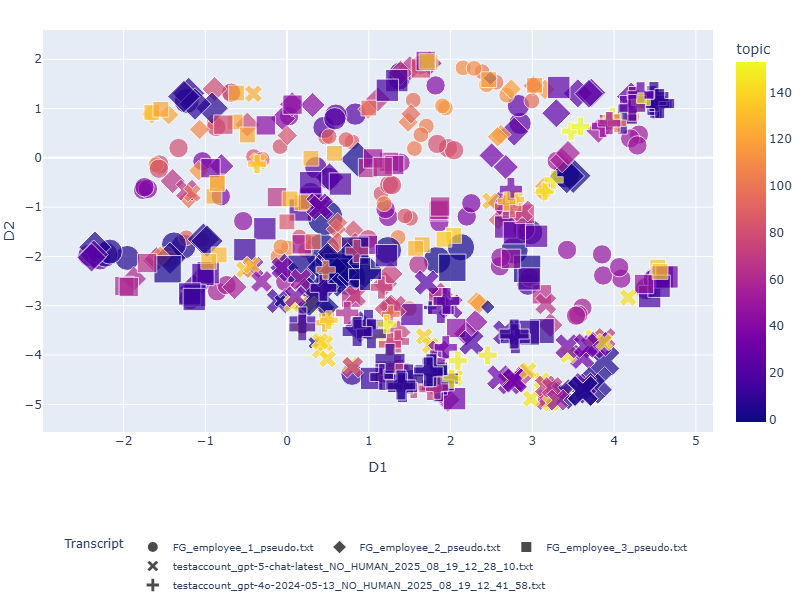
\includegraphics[keepaspectratio]{fig_chunks.png}}

}

\caption{\label{fig-heatmap}}

\end{figure}%

\begin{figure}

\centering{

\pandocbounded{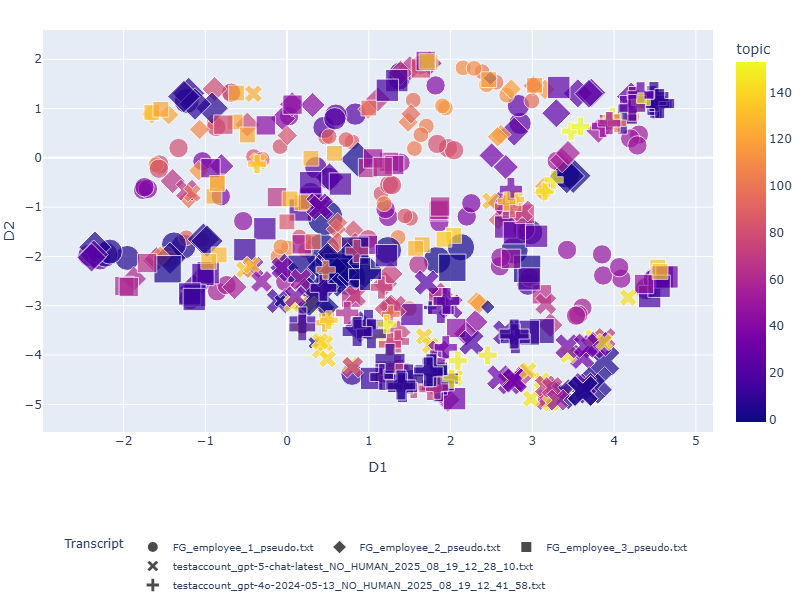
\includegraphics[keepaspectratio]{fig_chunks.png}}

}

\caption{\label{fig-chunks}}

\end{figure}%

\section{Conclusion}\label{sec-discussion}

\textbf{(4)} I coded a possible way how the moderator or system decides
on who is allowed to talk and who responds to others' comments.

\textbf{(5)} I coded a the possibility to simulate either some or all
participants of the focus-group with AI agents.

\textbf{(6)} I coded a way to publish the interview not only locally but
also publicly.

\textbf{(7)} I run a focus-group and compare the outcome of the given
outline with real world examples by embedding the real world example and
run a clustering exercise on both transcripts.

\textbf{How to determine whose turn it is to speak?}

Zum Beispiel über das andere Fokurgruppenpapier schrieben, dass meine
Transitionlogik natürlicher ist und diese auch noch weitere
Schwachstellen ausgemacht haben. Auch haben die im Gegensatz zu mir die
Messagestruktur anders genutzt, was ich etwas schwierig finde. Dazu
diskutieren. Auch diskutieren, dass man immer das Problem hat, ob man
Leute sehr strak oder praktisch gar nicht prompten soll. Das hat aber
trotzdem den Vorteil, dass das mit den unterschiedlichen Formen von
Fokusgruppen (Fachbereiche unter sich oder ganz unterschiedliche Leute
in einer Fokusgruppe) super kompatibel ist. Auch wenn es schwierig ist
bestimmte Charaktere zu bekommen, kann man die einfach mit AI Agenten
simulieren. Auch sich darauf beziehen, dass Leute gerne mit AIs
interagiere. Zukünftige Schritte wären Spracherweiterung und
Videosimulation der AI. Vorteil ist auch, dass AI Agents prinzipiell
keiner Sample Selection unterliegen, also sich nicht rausselektieren
können. Es ist allerdings die Frgae, ob so ein Verhalten vielleicht isch
auch in der Datenebene mit denen die AI Agenten trainiert sind
wiederspiegelt. Siehe Limitations von Morton et al.
(\citeproc{ref-morton_fitzsimons_sivaramakrishan_jepson_niven_2024}{2024}).

Für die Diskussion oder Conclusion verweise auch auf Zhang et al.
(\citeproc{ref-zhang_zhang_cools_simeone_2024}{2024}).

\section*{References}\label{sec:references}
\addcontentsline{toc}{section}{References}

\phantomsection\label{refs}
\begin{CSLReferences}{1}{0}
\bibitem[\citeproctext]{ref-bergman_chetty_deluca_hendren_katz_palmer_2024}
Bergman, Peter, Raj Chetty, Stefanie DeLuca, Nathaniel Hendren, Lawrence
F. Katz, and Christopher Palmer. 2024. {``{Creating Moves to
Opportunity: Experimental evidence on barriers to Neighborhood
Choice}.''} \emph{American Economic Review} 114 (5): 1281--1337.

\bibitem[\citeproctext]{ref-billups_2021}
Billups, Felice D. 2021. {``Focus Group Moderator Guides.''} \emph{Focus
Group Moderator Guides}, 97--132.

\bibitem[\citeproctext]{ref-braun_clarke_2021}
Braun, Virginia, and Victoria Clarke. 2021. {``Thematic Analysis: A
Practical Guide.''}

\bibitem[\citeproctext]{ref-bursztyn_haaland_roever_roth_2025}
Bursztyn, Leonardo, Ingar K Haaland, Nicolas Röver, and Christopher
Roth. 2025. {``The Social Desirability Atlas.''} National Bureau of
Economic Research.

\bibitem[\citeproctext]{ref-chopra_haaland_2024}
Chopra, Felix, and Ingar Haaland. 2024. {``{Conducting Interview with
AI}.''} \emph{Working Paper}.

\bibitem[\citeproctext]{ref-geiecke_jaravel_2025}
Geiecke, Friedrich, and Xavier Jaravel. 2025. {``{Conversations at
Scale: Robust AI-led Interviews}.''} \emph{Working Paper}.

\bibitem[\citeproctext]{ref-grootendorst_2022}
Grootendorst, Maarten. 2022. {``BERTopic: Neural Topic Modeling with a
Class-Based TF-IDF Procedure.''} \emph{arXiv Preprint arXiv:2203.05794}.

\bibitem[\citeproctext]{ref-haaland_roth_stantcheva_wohlfahrt_forthcoming}
Haaland, Ingar, Chris Roth, Stefanie Stantcheva, and Johannes Wohlfahrt.
forthcoming. {``{Understanding Economic Behavior Using Open-ended Survey
Data}.''} \emph{Journal of Economic Literature}, forthcoming.

\bibitem[\citeproctext]{ref-kahan_2001}
Kahan, James P. 2001. {``Focus Groups as a Tool for Policy Analysis.''}
\emph{Analyses of Social Issues and Public Policy} 1 (1): 129--46.

\bibitem[\citeproctext]{ref-morton_fitzsimons_sivaramakrishan_jepson_niven_2024}
Morton, Sarah, Claire Fitzsimons, Divya Sivaramakrishnan, Ruth Jepson,
and Ailsa Niven. 2024. {``{`Are We Working (Too) Comfortably?'}: A Focus
Group Study to Understand Sedentary Behaviour When Working at Home and
Identify Intervention Strategies.''} \emph{BMC Public Health} 24 (1):
1516.

\bibitem[\citeproctext]{ref-olawade_omeni_gore_hadi_2025}
Olawade, David B, Deborah Omeni, Manisha Nitin Gore, and Manizha Hadi.
2025. {``Enhancing Qualitative Research Through Virtual Focus Groups and
Artificial Intelligence: A Review.''} \emph{International Journal of
Medical Informatics}, 106004.

\bibitem[\citeproctext]{ref-rabiee_2004}
Rabiee, Fatemeh. 2004. {``Focus-Group Interview and Data Analysis.''}
\emph{Proceedings of the Nutrition Society} 63 (4): 655--60.

\bibitem[\citeproctext]{ref-zhang_zhang_cools_simeone_2024}
Zhang, Taiyu, Xuesong Zhang, Robbe Cools, and Adalberto Simeone. 2024.
{``Focus Agent: Llm-Powered Virtual Focus Group.''} In \emph{Proceedings
of the 24th ACM International Conference on Intelligent Virtual Agents},
1--10.

\end{CSLReferences}




\end{document}
